\documentclass[a4paper,10pt,twoside=semi,openany]{scrbook}
%\documentclass[a4paper,10pt]{scrartcl}

\usepackage{mystyle}

\title{Representation Theory I}
\author{Jendrik Stelzner}
\date{\today}

\begin{document}

\frontmatter
\maketitle
\chapter*{Preface}

The following are my personal notes about the representation theory of (semisimple) Lie algebras.
These notes were originally based on the lecture course \emph{Representation~Theory~I} that was given by Prof.~Dr.~Catharina Stroppel at the University of Bonn in the summer term~2015.
The notes are currently under heavy reconstruction.
If you have comments or corrections regarding these notes, feel free to contact me at \href{mailto:jendrikstelzner@uni-bonn.de}{jendrikstelzner@uni-bonn.de}.
You can also leave feedback at this project’s webpage at \url{https://gitlab.com/lecture-notes-bonn/lie-algebras}.

\tableofcontents

\mainmatter
\chapter{The Basics}
\section{Basic definitions}





\subsection{Definition and examples for Lie algebras}


\begin{defi}
 Let $\g$ be a vector space over some field $k$. A $k$-bilinear map
 \[
  [\cdot, \cdot] \colon \g \times \g \to \g
 \]
 is called a \emph{Lie bracket} if it satisfies the following two conditions:
 \begin{enumerate}
  \item
   $[\cdot, \cdot]$ is \emph{alternating}, i.e.\ $[x,x] = 0$ for every $x \in \g$.
  \item
   $[\cdot, \cdot]$ satisfies the \emph{Jacobi identity}
   \[
    [x,[y,z]] + [y,[z,x]] + [z,[x,y]] = 0
    \quad
    \text{for all $x,y,z \in \g$}.
   \]
 \end{enumerate}
 A $k$-vector space $\g$ together with the Lie-bracket $[\cdot,\cdot]$ is called a \emph{$k$-Lie algebra}.
\end{defi}


\begin{rem}
 Any Lie bracket $[\cdot, \cdot]$ is antisymmetric, i.e.\ $[y,x] = -[x,y]$ for all $x,y \in \g$, because
 \[
  0 = [x+y, x+y] = [x,x] + [x,y] + [y,x] + [y,y] = [x,y] + [y,x].
 \]
\end{rem}


\begin{rem}
 Using the antisymmetry of the Lie bracket the Jacobi identity can be rewritten as
 \[
  [x,[y,z]] = [[x,y],z] + [y,[x,z]] \quad \text{for all $x,y,z \in \g$}.
 \]
\end{rem}



\begin{expls}
 \begin{enumerate}[leftmargin=*]
  \item
   Any vector space $V$ becomes a Lie algebra via
   \[
    [x,y] = 0 \quad \text{for all $x,y \in V$}.
   \]
  \item
   Any \emph{associative} $k$-algebra $A$ becomes a Lie algebra via
   \[
    [a,b] = ab-ba \quad \text{for all $a,b \in A$}.
   \]
   It is clear that $[\cdot, \cdot]$ is alternating and because $A$ is associative it follows that for all $a,b,c \in A$
   \begin{align*}
    &\, [a,[b,c]] + [b,[c,a]] + [c,[a,b]] \\
    &= [a, (bc-cb)] + [b, (ca-ac)] + [c, (ab-ba)] \\
    &= a(bc-cb)-(bc-cb)a + b(ca-ac) - (ca-ac)b + c(ab-ba) - (ab-ba)c \\
    &= abc -acb -bca +cba +bca -bac -cab +acb +cab -cba -abc +bac \\
    &= 0.
   \end{align*}
   
   The following two are important examples of this construction:
   \begin{enumerate}
    \item
     The $k$-algebra of ($n \times n$)-matrices $\Mat_n(k)$ becomes a Lie algebra via
     \[
      [A,B] = AB-BA \quad \text{for all $A,B \in \Mat_n(k)$}.
     \]
     This is called the \emph{general linear Lie algebra} and is denoted by $\gl_n(k)$.
    \item
     More generally for any $k$-vector space the $k$-algebra $\End_k(V)$ becomes a Lie algebra via
     \[
      [\varphi_1, \varphi_2] \coloneqq \varphi_1 \circ \varphi_2 - \varphi_2 \circ \varphi_1
      \quad
      \text{for all $\varphi_1, \varphi_2 \in \End_k$}.
     \]
     This is called the \emph{general linear Lie algebra for $V$} and is denoted by $\gl(V)$.
   \end{enumerate}
 \end{enumerate}
\end{expls}


\begin{defi}
 Let $\g$ be a $k$-Lie algebra. A \emph{Lie subalgebra} of a $\g$ is a $k$-linear subspace $\h \subseteq \g$ such that
 \[
  [x,y] \in \h \quad \text{for all $x,y \in \h$}.
 \]
 An \emph{ideal} inside $\g$ is a $k$-linear subspace $I \subseteq \g$ such that
 \[
  [x,y] \in I \quad \text{for all $x \in \g$ and $y \in I$}.
 \]
 That $I$ is an ideal in $\g$ is denoted by $I \subideal \g$.
\end{defi}


\begin{rem}
 It is not necessary to distinguish between left ideals or right ideals in a Lie algebra because the Lie bracket is antisymmetric.
\end{rem}


\begin{rem}
 For a Lie algebra $\g$ and a subalgebra $\h \subseteq \g$ it follows that $\h$ becomes a Lie algebra by restricting the Lie bracket of $\g$ to $\h$. Every ideal inside $\g$ is also a subalgebra of $\g$.
\end{rem}


\begin{defi}
 Let $\g$ be a Lie algebra. The \emph{center} of $\g$ is
 \[
  Z(\g) \coloneqq \{x \in \g \mid \text{$[x,y] = 0$ for every $y \in \g$}\}
 \]
 $\g$ is called \emph{abelian} if $Z(\g) = 0$, i.e.\ if $[x,y] = 0$ for all $x,y \in \g$.
\end{defi}


\begin{defi}
 For a Lie-algebra $\g$ over some field $k$ and subsets $X, Y \subseteq \g$ let
 \[
  [X,Y] \coloneqq \vspan_k \{[x,y] \mid x \in X, y \in Y\}.
 \]
\end{defi}


\begin{rem}
 Clearly $\g$ is abelian if and only if $[\g,\g] = 0$. Also notice that $[\g,\g]$ and $Z(\g)$ are ideals inside $\g$.
\end{rem}


\begin{lem}
 Let $\g$ be a Lie algebra over some field $k$.
 \begin{enumerate}[leftmargin=*]
  \item
   If $I_\lambda$, $\lambda \in \Lambda$ is a collection of ideals $I_\lambda \subideal \g$ then also $\bigcap_{\lambda \in \Lambda} I_\lambda \subideal \g$ and $\sum_{\lambda \in \Lambda} I_\lambda \subideal \g$.
  \item
   If $I, J \subideal \g$ then also $[I,J] \subideal \g$.
 \end{enumerate}
\end{lem}
\begin{proof}
 \begin{enumerate}[leftmargin=*]
  \item
   This follows from direct calculation.
  \item
   As $[I,J]$ is spanned by the elements $[y,z]$ with $y \in I$ and $z \in J$ it is enough to show that $[x,[y,z]] \in [I,J]$ for every $x \in \g$, $y \in I$ and $z \in J$. This follows from $I, J \subideal \g$ and the Jacobi identity, because
   \[
    [x,[y,z]]
    = [\underbrace{[x,y]}_{\in I},z] + [y,\underbrace{[x,z]}_{\in J}]
    \in [I,J].
   \qedhere
   \]
 \end{enumerate}
\end{proof}


\begin{defi}
 A Lie algebra $\g$ is called \emph{linear} if $\g$ is a Lie subalgebra of $\gl(V)$ for some finite dimensional vector space $V$.
\end{defi}


\begin{expl}
 \begin{enumerate}[leftmargin=*]
  \item
   Let $\g = \gl_n(k)$. Then
   \begin{gather*}
     \sll_n(k) = \{A \in \g \mid \tr A = 0\}
   \shortintertext{is an ideal in $\g$ because}
     \sll_n(k) = [\g,\g].
   \end{gather*}
   To see this first notice that on the one hand
   \[
     \tr [A,B]
     = \tr(AB-BA)
     = \tr(AB) - \tr(BA)
     = \tr(AB) - \tr(AB)
     = 0
   \]
   for all $A, B \in \g$ and therefore $[\g,\g] \subseteq \sll_n(k)$.
   
   On the other hand notice that $\sll_n(k)$ has a basis given by the elementary matrices $e_{ij}$ with $1 \leq i \neq j \leq n$ and $e_{11} - e_{ii}$ with $i = 2, \dotsc, n$. Each of these matrices is given as a commutator, namely $e_{ij} = [e_{ii},e_{ij}]$ for $1 \leq i \neq j \leq n$ and $e_{11} - e_{ii} = [e_{1i},e_{i1}]$ for $i = 2, \dotsc, n$. Therefore $\sll_n(k) \subseteq [\g,\g]$.
   
  \item
   The upper triangular matrices
   \[
    \tl_n(k) \coloneqq
    \left\{
     \begin{pmatrix}
      a_{11} & \cdots & \cdots & a_{1n} \\
           0 & \ddots &        & \vdots \\
      \vdots & \ddots & \ddots & \vdots \\
           0 & \cdots &      0 &  a_{nn}
     \end{pmatrix}
     \,\middle|\,
     \text{$a_{ij} \in k$ for every $1 \leq i \leq j \leq n$}
    \right\}
   \]
   are a Lie subalgebra of $\gl_n(k)$.
   
  \item
   The strictly upper triangular matrices
   \[
    \nl_n(k) \coloneqq
    \left\{
     \begin{pmatrix}
           0 & a_{12} & \cdots &    a_{1n} \\
      \vdots & \ddots & \ddots &    \vdots \\
      \vdots &        & \ddots & a_{n-1,n} \\
           0 & \cdots & \cdots &         0   
     \end{pmatrix}
     \,\middle|\,
     \text{$a_{ij} \in k$ for every $1 \leq i < j \leq n$}
    \right\}
   \]
   are a Lie subalgebra of $\tl_n(k)$ and therefore also of $\gl_n(k)$. It is even an ideal in $\tl_n(k)$ because $\nl_n(k) = [\tl_n(k), \tl_n(k)]$.
 \end{enumerate}
\end{expl}





\subsection{Homomorphisms of Lie algebras}


\begin{defi}
 Given Lie algebras $\g_1$ and $\g_2$ over the same field $k$ a \emph{homomorphism of Lie algebras} $\g_1 \to \g_2$ is a $k$-linear map $f \colon \g_1 \to \g_2$ such that
 \[
  f([x,y]) =[f(x),f(y)] \quad \text{for all $x,y \in \g_1$}.
 \]
\end{defi}


\begin{expls}
 \begin{enumerate}[leftmargin=*]
  \item
   For any Lie algebra $\g$ the identity $\id_\g \colon \g \to \g$ is a Lie algebra homomorphism.
  \item
   Given Lie algebras $\g_1$, $\g_2$ and $\g_3$ and Lie algebra homomorphisms $f_1 \colon \g_1 \to \g_2$ and $f_2 \colon \g_2 \to \g_3$ the composition $f_2 \circ f_1 \colon \g_1 \to \g_3$ is also a homomorphism of Lie algebras.
  \item
   If $\g$ is a Lie algebra and $\h \subseteq \g$ a Lie subalgebra then the inclusion $\h \inc \g$ is a homomorphism of Lie algebras.
 \end{enumerate}
\end{expls}


\begin{defi}
 Let $\g_1, \g_2$ be Lie algebras over the same field $k$. A homomorphism of Lie algebras $f \colon \g_1 \to \g_2$ is called an \emph{isomorphism of $k$-Lie algebras} if $f$ is bijective.
\end{defi}


\begin{lem}
 If $f \colon \g_1 \to \g_2$ is an isomorphism of $k$-Lie algebras, then the $k$-linear map $f^{-1} \colon \g_2 \to \g_1$ is also a homomorphism of Lie-algebras and therefore also an isomorphism.
\end{lem}
\begin{proof}
 For all $x,y \in \g_2$
 \begin{align*}
  f^{-1}( [x,y] )
  &= f^{-1}( [ f(f^{-1}(x)), f(f^{-1}(y)) ] ) \\
  &= f^{-1}(f( [f^{-1}(x) , f^{-1}(y)] )) \\
  &= [f^{-1}(x), f^{-1}(y)].
 \qedhere
 \end{align*}
\end{proof}


\begin{rem}
 It follows that Lie algebras over the same field $k$ together with homomorphisms of Lie algebras and their usual composition form a category. An \emph{isomorphism of $k$-Lie algebras} is an isomorphism in the category of $k$-Lie algebras.
\end{rem}


We have the usual theorems about homomorphisms and ideals.


\begin{prop}
 Let $\g_1$ and $\g_2$ be Lie algebras and $f \colon \g_1 \to \g_2$ a homomorphism of Lie algebras.
 \begin{enumerate}[leftmargin=*]
  \item
   $\ker f \subideal \g_1$ is an ideal.
  \item
   $\im f \subseteq \g_2$ is a Lie subalgebra.
  \item
   If $I \subideal \g_1$ is an ideal with $\ker f \subseteq I$ then there exists a unique homomorphism of Lie algebras $\tilde{f} \colon \g_1/I \to \g_2$ with $f = \tilde{f} \circ \pi$ where $\pi \colon \g_1 \to \g_1/I$ is the canonical projection.
   \tikzsetnextfilename{universal_property_of_quotient_of_lie_algebras}
   \begin{center}
    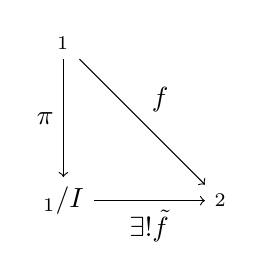
\begin{tikzpicture}[node distance = 2cm]
     \node (g1) {$\g_1$};
     \node (gI) [below of = g1] {$\g_1/I$};
     \node (g2) [right of = gI] {$\g_2$};
     \draw[->] (g1) to node[above right] {$f$} (g2);
     \draw[->] (g1) to node[left] {$\pi$} (gI);
     \draw[->] (gI) to node[below] {$\exists! \tilde{f}$} (g2);
    \end{tikzpicture}
   \end{center}
  \item
   If $I, J \subideal \g$ are subideals with $I \subseteq J$ then $J/I \subideal \g/I$ and the natural isomorphism of vector spaces
   \[
    (\g/I)/(J/I) \to \g/I, \quad (x+I)+(J/I) \mapsto x+I
   \]
   is already a natural isomorphism of Lie algebras.
  \item
   If $I, J \subideal \g$ are subideals then the natural isomorphism of vector spaces
   \begin{gather*}
    (I + J)/J \to I/(I \cap J)
   \shortintertext{defined by}
    (x+J)+I \mapsto x + (I \cap J) \quad \text{for every $x \in I$}
   \end{gather*}
   is already a natural isomorphism of Lie algebras.
 \end{enumerate}
\end{prop}


\begin{rem}
 For a Lie algebra $\g$ the ideal $[\g,\g]$ is the minimal ideal inside $\g$ such that $\g/[\g,\g]$ is abelian. Furthermore given any abelian Lie algebra $\h$ any homomorphism of Lie algebras $\g \to \h$ factorizes through a unique homomorphism of Lie algebras $\g/[\g,\g] \to \h$.
 \begin{center}
  \tikzsetnextfilename{universal_property_of_abelization}
  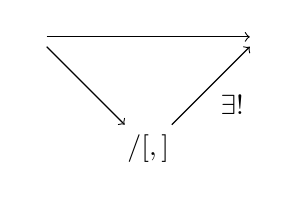
\begin{tikzpicture}[node distance = 2cm]
   \node (gab) {$\g/[\g,\g]$};
   \node (g) [above left of = gab] {$\g$};
   \node (h) [above right of = gab] {$\h$};
   \draw[->] (g) to (h);
   \draw[->] (g) to (gab);
   \draw[->] (gab) to node[below right] {$\exists!$} (h);
  \end{tikzpicture}
 \end{center}
\end{rem}




\subsection{New Lie algebras from old ones}


\begin{defi}
 Let $\g_1$ and $\g_2$ be Lie algebras over the same field $k$. Then the \emph{product} of $\g_1$ and $\g_2$ is defined as the $k$-vector space $\g_1 \times \g_2$ together with the Lie bracket
 \[
  [(x_1, y_1), (x_2, y_2)]
  = ([x_1, x_2], [y_1, y_2])
  \quad
  \text{for all $(x_1, y_1), (x_2, y_2) \in \g_1 \times \g_2$}.
 \]
\end{defi}


\begin{defi}
 Let $\g$ be a Lie algebra and $I \subideal \g$. Then the induced Lie algebra structure on the quotient vector space $\g/I$ is given by
 \[
  [x+I, y+I] = [x,y] + I \quad \text{for all $x,y \in \g$}.
 \]
\end{defi}


\begin{rem}
 The Lie algebra structure on the quotient $\g/I$ is well-defined: If $x,y, x',y' \in \g$ with $x+I = x'+I$ and $y+I = y'+I$ then $x-x' \in I$ and $y-y' \in I$ and thus
 \begin{align*}
  [x,y] + I
  &= [x' + x-x', y' + y-y'] + I \\
  &= [x',y'] + \underbrace{[x', y-y']}_{\in I} + \underbrace{[x-x', y']}_{\in I} + \underbrace{[x-x', y-y']}_{\in I} + I
  = [x', y'] + I.
 \end{align*}
 The additional properties of a Lie bracket follows from the Lie bracket of $\g$ safisfying them.
\end{rem}


\begin{lem}
 \begin{enumerate}[leftmargin=*]
  \item
   If $\g_1$ and $\g_2$ are Lie algebras then the canonical projections
   \[
    \pi_i \colon \g_1 \times \g_2 \to \g_i, \quad (x_1, x_2) \mapsto x_i
    \quad \text{for $i = 1, 2$}
   \]
   are homomorphisms of Lie-algebras.
  \item
   If $\g$ is a Lie algebra and $I \subideal \g$ then the canonical projection $\pi \colon \g \to \g/I, x \mapsto [x]$ is a homomorphism of Lie algebras.
 \end{enumerate}
\end{lem}



\begin{lem}\label{lem: quasi extension of scalars for Lie algebras}
Let $\g$ be a Lie algebra over $k$ and $A$ an associative, commutative $k$-algebra. Then $A \otimes_k \g$ is a Lie algebra over $k$ via
\[
 [a \otimes x, b \otimes y] = (ab) \otimes [x,y]
 \quad
 \text{for all $a,b \in A$ and $x,y \in \g$}.
\]
Similarly $\g \otimes_k A$ carries the structure of a Lie algebra over $k$ via
\[
 [x \otimes a, y \otimes b] = [x,y] \otimes (ab)
 \quad
 \text{for all $x,y \in \g$ and $a,b \in A$}.
\]
\end{lem}


\begin{expl}
 If $L/k$ is a field extension and $\g$ a Lie algebra over $k$, then $L \otimes_k \g$ is a Lie algebra over $k$ via
 \[
  [\lambda \otimes x, \mu \otimes y] = (\lambda \mu) \otimes [x,y]
  \quad
  \text{for alle $\lambda, \mu \in k$ and $x,y \in \g$}.
 \]
 $L \otimes_k \g$ also carries the structure of an $L$-vector space via extension of scalars, i.e.
 \[
  \lambda \cdot (\mu \otimes x) = (\lambda \mu) \otimes x
  \quad
  \text{for alle $\lambda, \mu \in k$ and $x \in \g$},
 \]
 and the Lie bracket is not only $k$-bilinear, but also $L$-bilinear. Hence the structure of a $k$-Lie algebra on $L \otimes_k \g$ can be extended to the structure of a Lie algebra over $L$. (Notice that the Jacobi-Identity is independent of the ground field.)
\end{expl}


\begin{defi}
 Let $\g$ be a Lie algebra and $A = k[t,t^{-1}]$ be the algebra of Laurent polynomials over $k$. Then
 \[
  \Loop(\g) \coloneqq \g \otimes_k A
 \]
 with the Lie bracket as in Lemma \ref{lem: quasi extension of scalars for Lie algebras} is called the \emph{loop (Lie) algebra} of $\g$.
\end{defi}


Another example for constructing new Lie algebras out of old ones are \emph{central extensions}: Let $\g$ be any $k$-Lie algebra.
\[
 \tilde{\g}
 \coloneqq \g \oplus k
 = \{x + \lambda c \mid x \in \g, \lambda \in k\},
\]
where we understand $c$ as a formal variable. Suppose that $\kappa \colon \g \times \g \to k$ is a $k$-bilinear map satisfying the following properties:
\begin{enumerate}
 \item
  $\kappa$ is antisymmetric, i.e.\ $\kappa(x,y) = -\kappa(y,x)$ for all $x,y \in \g$.
 \item
  $\kappa$ satisfies the $2$-cocycle condition
  \[
   \kappa([x,y],z) + \kappa([y,z],x) + \kappa([z,x],y) = 0
   \quad
   \text{for all $x,y,z \in \g$}.
  \]
\end{enumerate}
Then $\tilde{\g}$ becomes a Lie algebra via
\[
 [x + \lambda c, y + \mu c] \coloneqq [x,y] + \kappa(x,y) \lambda \mu c
 \quad \text{for all $x,y \in \g$ and $\lambda, \mu \in k$.}
\]
Note that $c$ is central in $\tilde{\g}$ in the sense that $[x,c] = 0$ for all $x \in \g$.


\begin{expl}
 Let $\g = \gl_n(k)$. We define a symmetric bilinear form on $\g$ via
 \[
  (A,B)_{\tr} = \tr(AB) \quad \text{for all $A,B \in \g$}.
 \]
 We define a bilinear form
 \[
  \Loop(\g) \times \Loop(\g) \to k[t,t^{-1}], \quad
  (x \otimes p, y \otimes q) \mapsto (x,y)_{\tr}\ pq
 \]
 We now get a $2$-cocycle $\kappa \colon \Loop(\g) \times \Loop(\g) \to k$ via
 \[
  \kappa(a,b) \coloneqq \mathrm{Res}\left(\frac{\partial a}{\partial t}, b\right).
 \]
 $\kappa$ is also antisymmetric: Let $a = x \otimes t^i$ and $b = y \otimes t^j$ with $x,y \in \g$ and $i,j \in \Z$. Then
 \begin{align*}
  \kappa(x \otimes t^i, y \otimes t^j)
  = \mathrm{Res}(i x \otimes t^{i-1}, y \otimes t^j)
  &= \mathrm{Res}(i t^{i+j-1} (x,y)_{\tr}) \\
  &=
  \begin{cases}
   i (x,y)_{\tr} & \text{if $i+j = 0$}, \\
               0 & \text{otherwise}.
  \end{cases}
 \end{align*}
 In the same way we find that
 \[
  \kappa(y \otimes t^j, x \otimes t^i) =
  \begin{cases}
   j (x,y)_{\tr} & \text{if $i+j = 0$}, \\
               0 & \text{otherwise}.
  \end{cases}
 \]
 Since $(\cdot,\cdot)_{\tr}$ is symmetric we find that
 \begin{align*}
  \kappa(x \otimes t^i, y \otimes t^j)
  &=
  \begin{cases}
   i (x,y)_{\tr} & \text{if $i+j = 0$}, \\
               0 & \text{otherwise},
  \end{cases} \\
  &=
  \begin{cases}
   -j (x,y)_{\tr} & \text{if $i+j = 0$}, \\
                0 & \text{otherwise},
  \end{cases} \\
  &=
  -\kappa(y \otimes t^j, x \otimes t^i).
 \end{align*}
\end{expl}





\subsection{Derivations}


\begin{defi}
 Let $A$ be a $k$-algebra (not necessarily unitary of even associative). A \emph{derivation of $A$} is a $k$-linear map $d \colon A \to A$ such that
 \[
  d(ab) = d(a)b + ad(b) \quad \text{for all $a,b \in A$}.
 \]
 We set
 \[
  \Der(A) \coloneqq \{d \colon A \to A \mid \text{$d$ is a derivation of $A$} \}.
 \]
\end{defi}


\begin{rem}
 $\Der(A)$ is a $k$-linear subspace of $\End_k(A)$.
\end{rem}


\begin{expl}
  Let $A$ be a $k$-algebra. It follows from direct calculation that for all $d, d' \in \Der(A)$ the commutator $[d,d'] = d \circ d' - d' \circ d$ is again a derivation $\Der(A)$. Hence $\Der(A)$ is a Lie subalgebra of $\gl(A)$.
\end{expl}


\begin{defi}
 Let $\g$ be a Lie algebra. Then
 \[
  \ad \colon \g \to \gl(\g), \quad x \mapsto [x,\cdot]
 \]
 is called the \emph{adjoint representation} of $\g$.
\end{defi}


\begin{lem}\label{lem: Lie algebras act adjoint by derivations}
 Let $\g$ be a Lie algebra. Then for any $x \in \g$ the map $\ad(x) \colon \g \to \g$ is a derivation of $\g$.
\end{lem}
\begin{proof}
 By the Jacobi identity
 \begin{align*}
  \ad(x)([y,z])
  &= [x,[y,z]]
  = [[x,y],z] + [y,[x,z]] \\
  &= [\ad(x)(y),z] + [y,\ad(x)(z)]
 \end{align*}
 for all $y,z \in \g$.
\end{proof}


\begin{defi}
 Let $\g$ be a Lie algebra. A derivation of $\g$ is called \emph{inner} if it is of the form $\ad(x)$ for some $x \in \g$.
\end{defi}


\begin{lem}
 If $\g$ is a Lie algebra then the inner derivations form an ideal inside of $\Der(\g)$.
\end{lem}
\begin{proof}
 Let $I \coloneqq \im \ad \subseteq \Der(\g)$ be the linear subspace of inner derivations. For any $\delta \in \Der$ and $x \in \g$ it follows that for any $y \in \g$
 \begin{align*}
  &\,[\delta, \ad(x)](y)
  = (\delta \ad(x) - \ad(x) \delta(x))(y) \\
  &= \delta([x,y]) - [x,\delta(y)]
  = [\delta(x),y] + [x,\delta(y)] - [x,\delta(y)] \\
  &= [\delta(x),y]
  = \ad(\delta(x))(y).
 \end{align*}
 Hence $[\delta, \ad(x)] = \ad(\delta(x)) \in I$.
\end{proof}










\subsection{Representations of Lie algebras}



\subsubsection{Definition of a representation}


\begin{defi}
 Let $\g$ be a $k$-Lie algebra. A \emph{representation} of $\g$ is a $k$-vector space $V$ together with a homomorphism of Lie algebras $\rho \colon \g \to \gl(V)$. This representation is called \emph{faithful} if $\rho$ is injective. The \emph{dimension} of this representation is the dimension of $V$.
\end{defi}


\begin{rem}
 Equivalently a representation of $\g$ is a $k$-vector space $V$ together with a $k$-bilinear map $\g \times V \to V, (x,v) \mapsto x.v$ such that
 \[
  x.(y.v) - y.(x.v) = [x,y].v \quad \text{for all $x,y \in \g$ and $v \in V$}.
 \]
 We will not distinguish between these two concepts and choose whichever is more useful in the given situation.
\end{rem}


\begin{defi}
 Let $V$ und $W$ be representations of a $k$-Lie algebra $\g$. A $k$-linear map $f \colon V \to W$ is called a \emph{homomorphism of representations} if
 \[
  f(x.v) = x.f(v) \quad \text{for every $x \in \g$ and $v \in V$}.
 \]
 If $\rho_V \colon \g \to \gl(V)$ and $\rho_W \colon \g \to \gl(W)$ are the corresponding Lie algebra homomomorphisms this is equivalent to
 \[
  f \circ \rho_V(x) = \rho_W(x) \circ f \quad \text{for every $x \in X$}.
 \]
 $f$ is an \emph{isomorphism of representations} if it is additionally bijective.
\end{defi}


\begin{rem}
 If $f \colon V \to W$ is an isomorphism of representations of a Lie algebra $\g$ then the $k$-linear map $f^{-1} \colon W \to V$ is also a homomorphism of representations (and therefore an isomorphism of representations) because
 \[
  f^{-1}(x.v) = f^{-1}(x.f(f^{-1}(v))) = f^{-1}(f(x.f^{-1}(v))) = x.f^{-1}(v)
 \]
 for every $x \in \g$ and $v \in V$. It also follows for every $x \in \g$ from $f \rho_V(x) = \rho_W(x) f$ that $\rho_V(x) f^{-1} = f^{-1} \rho_W(x)$.
\end{rem}





\subsubsection{The adjoint representation}


\begin{expl}
 For any Lie algebra $\g$ the adjoint representation $\ad \colon \g \to \gl(V)$ is a representation of $\g$: That $\ad$ is a homomorphism of Lie algebras is equivalent to
 \begin{gather*}
  \ad([x,y])(z) = [\ad(x),\ad(y)](z) \quad \text{for all $x,y,z \in \g$}.
 \shortintertext{Because}
  \ad([x,y])(z) = [[x,y],z] = -[z,[x,y]]
 \shortintertext{and}
  \begin{aligned}
   [\ad(x),\ad(y)](z)
   &= (\ad(x) \circ \ad(y))(z) - (\ad(y) \circ \ad(x))(z) \\
   &= [x,[y,z]] - [y,[x,z]]
   = [x,[y,z]] + [y,[z,x]]
  \end{aligned}
 \end{gather*}
 this is equivalent to the Jacobi identity. Hence $\ad$ really is a representation of $\g$.
 
 Together with Lemma \ref{lem: Lie algebras act adjoint by derivations} it follows that $\g$ acts on itself by derivations of itself.

 As $\ker \ad = Z(\g)$ the adjoint representation is faithful if and only if $Z(\g) = 0$.
\end{expl}


\begin{expl}
 If $\g \subseteq \gl(V)$ is a Lie subalgebra then $V$ is a representation of $\g$ via the inclusion $\g \inc \gl(V)$. This corresponds to the action
 \[
  x.v = x(v) \quad \text{for every $x \in \g$ and $v \in V$}.
 \]
\end{expl}



\subsubsection{New representations from old ones}


\begin{prop}
 Let $\g$ be a Lie algebra over a field $k$.
 \begin{enumerate}[leftmargin=*]
  \item
   If $(V_i)_{i \in I}$ is a collection of representations of $\g$ then $\bigoplus_{i \in I} V_i$ is a representation of $\g$ via
   \[
    x.\sum_{i \in I} v_i = \sum_{i \in I} x.v_i
   \]
   or every $x \in \g$ and $v_i \in V_i$ for all $i \in I$, with $v_i = 0$ for all but finitely many $i \in I$.
  \item
   If $V$ and $W$ are representations of $\g$ then $V \otimes W$ is a representation of $\g$ via
   \[
    x.(v \otimes w) = (x.v) \otimes w + v \otimes (x.w) \quad \text{for every $x \in \g$, $v \in V$ and $w \in W$}.
   \]
   More generally: If $V_1, \dotsc V_n$ are representations of $\g$ then $\bigotimes_{i=1}^n V_i$ is a representation of $\g$ via
   \[
    x.(v_1 \otimes \dotsb \otimes v_n)
    = \sum_{i=1}^n v_1 \otimes \dotsb \otimes v_{i-1} \otimes (x.v_i) \otimes v_{i+1} \otimes \dotsb \otimes v_n.
   \]
   for every $x \in \g$ and $v_i \in V_i$ for every $i = 1, \dotsc, n$.
  \item
   If $V, W$ are representations of $V$ then $\Hom_k(V,W)$ is a representation of $\g$ via
   \[
    (x.f)(v) = x.f(v) - f(x.v) \quad \text{for every $x \in \g$, $f \in \Hom(V,W)$ and $v \in V$}.
   \]
  \item
   By letting $\g$ act trivially on $k$ the dual $V^* = \Hom_k(V,k)$ becomes a representation of $\g$ in the above way, i.e.
   \[
    (x.\varphi)(v) = -\varphi(x.v) \quad \text{for every $x \in \g$, $\varphi \in V^*$ and $v \in V$}.
   \]
 \end{enumerate}
\end{prop}


\begin{prop}
 Let $\g$ be a Lie algebra.
 \begin{enumerate}[leftmargin=*]
  \item
   If $V$ and $W$ are finite dimensional representations of $\g$ then the map
   \[
    V^* \otimes W \to \Hom_k(V,W), \quad \varphi \otimes w \mapsto (v \mapsto \varphi(v) w)
   \]
   is a homomorphism of representations. If $V$ and $W$ are both finite dimensional this is an isomorphism of vector spaces and thus already an isomorphism of representations.
  \item
   If $V^i_j$ with $i = 1, \dotsc, r$ and $j = 1, \dotsc, n_i$ is a collection of representations of $\g$ then the isomorphism of vector spaces
   \begin{align*}
    \bigotimes_{i=1}^r \bigotimes_{j=1}^{n_j} V^{i}_j
    &\to V^1_1 \otimes \dotsb \otimes V^1_{n_1} \otimes \dotsb \otimes V^r_1 \otimes \dotsb \otimes V^{r}_{n_r}, \\
    (v^1_1 \otimes \dotsb \otimes v^1_{n_1}) \otimes \dotsb \otimes (v^r_1 \otimes \dotsb \otimes v^r_{n_r})
    &\mapsto v^1_1 \otimes \dotsb \otimes v^1_{n_1} \otimes \dotsb \otimes v^r_1 \otimes \dotsb \otimes v^r_{n_r}
   \end{align*}
   is already an isomorphism of representations.
  \item
   If $V_1, \dotsc, V_n$ and $W_1, \dotsc, W_n$ are representations of $\g$ and $f_i \colon V_i \to W_i$ for every $i = 1, \dotsc, n$ a homomorphism of representations it follows that the map
   \[
    f_1 \otimes \dotsb \otimes f_n \colon \bigotimes_{i=1}^n V_i \to \bigotimes_{i=1}^n W_i,
    v_1 \otimes \dotsb \otimes v_n \mapsto f(v_1) \otimes \dotsb \otimes f(v_n)
   \]
   is also a homomorphism of representations.
 \end{enumerate}
\end{prop}


\subsubsection{Subrepresentations and irreducible representations}


\begin{defi}
 Let $\g$ be a Lie algebra and $\rho \colon \g \to \gl(V)$ a representation of $\g$. A \emph{subrepresentation} of $V$ is a linear subpace $U \subseteq V$ such that $x.u \in U$ for every $x \in \g$ and $u \in U$. Equivalently $U$ is $\rho(x)$ invariant for every $x \in \g$.
 
 If $(U_i)_{i \in I}$ is a collection of subrepresentations of $\g$ then $V$ is called the \emph{direct sum} of the $U_i$ if $V = \bigoplus_{i \in I} U_i$ as vector spaces.
\end{defi}


\begin{expls}
 Let $\g$ be a Lie algebra.
 \begin{enumerate}[leftmargin=*]
  \item
   If $V$ is a representation of $\g$ then $0$ and $V$ itself are subrepresentations. These are also called the \emph{trivial subrepresentations}.
  \item
   If $V$ is a representation and $(U_i)_{i \in I}$ a collection of subrepresentations $U_i \subseteq V_i$ then $\sum_{i \in I} U_i$ is also a subrepresentation of $V$.
  \item
   The subrepresentations of the adjoint representation of $\g$ are precisely the ideals in $\g$.
 \end{enumerate}
\end{expls}


\begin{defi}
 A representation $V$ of a Lie algebra $\g$ is called \emph{irreducible} if it has precisely two subrepresentations. Equivalently $V$ is nonzero and has only the trivial subrepresentations.
 
 $V$ is called \emph{decomposable} if there exist non-trivial subrepresentations $U_1, U_2 \subseteq V$ with $V = U_1 \oplus U_2$. Otherwise $V$ is called \emph{indecomposable}.
\end{defi}


\begin{rem}
 By definition every irreducible representation is also indecomposable. The converse does not hold.
\end{rem}



\begin{expl}
 The adjoint representation of a Lie algebra $\g$ is irreducible if and only if $\g \neq 0$ and $\g$ has no ideals besides $0$ and $\g$ itself. So $\g$ is either the onedimensional abelian Lie algebra or a simple Lie algebra.
\end{expl}







\subsection{Simple Lie algebras}


\begin{defi}
 A Lie algebra $\g$ is \emph{simple} if $0$ and $\g$ are the only ideals inside $\g$ and $\g$ is not abelian.
\end{defi}


\begin{lem}
 Let $\g$ be a simple Lie algebra. Then $[\g,\g] = \g$ and $Z(\g)=0$.
\end{lem}
\begin{proof}
 Because $\g$ is simple it is not abelian. Therefore $[\g,\g] \neq 0$ and $Z(\g) \neq \g$. Since $[\g,\g]$ and $Z(\g)$ are ideals inside $\g$ it follows that $[\g,\g] = \g$ and $Z(\g) = 0$.
\end{proof}


\begin{cor}
 Let $\g$ be simple. Then $\ad \colon \g \to \gl(\g)$ is injective. In particular $\g$ can be realized as a linear Lie algebra.
\end{cor}
\begin{proof}
 This directly follows from $\ker \ad = Z(\g) = 0$.
\end{proof}


It can be shown that every finite dimensional Lie algebra can be realized as a linear Lie algebra. This will not be proven in this lecture and is by far not trivial.


\begin{thrm}[Ado]
 Every finite dimensional Lie algebra $\g$ is isomorphic to a linear Lie algebra (which is equivalent to $\g$ having a faithful finite-dimensional representation).
\end{thrm}


\begin{expls}
 \begin{enumerate}[leftmargin=*]
  \item
   Since $[\gl_n(k),\gl_n(k)] = \sll_n(k) \neq \gl_n(k)$ we find that $\gl_n(k)$ is not simple.
  \item
   Let $\g = \sll_2(k)$. Then $\g$ is simple if and only if $\chara k \neq 2$. To see this consider the basis $(e,h,f)$ of $\sll_2(k)$ consisting of the matrices
   \[
    e = \begin{pmatrix}0 & 1 \\ 0 & 0\end{pmatrix}, \quad
    h = \vect{1 & 0 \\ 0 & -1}, \quad
    f = \vect{0 & 0 \\ 1 & 0}.
   \]
   of $\sll_2(k)$. Then
   \[
    [h,e] = 2e, \quad
    [h,f] = -2f, \quad
    [e,f] = h.
   \]
   If $\chara k = 2$ then $h$ spans a $1$-dimensional ideal, thus $\sll_2(k)$ is not simple. Suppose that $\chara k \neq 2$ and let $I \subseteq \sll_2(k)$ be an ideal with $I \neq 0$. It is clear that if $I$ contains one of the basis vectors $e$, $h$ or $f$ it follows that $I = \sll_2(k)$. Let $x \in I$ with $x \neq 0$ and write $x = \alpha e + \beta h + \gamma f$. Then
   \[
    [e,x] = -2 \beta e + \gamma h \quad \text{and} \quad [e,[e,x]] = -2 \gamma e.
   \]
   Since $\gamma = 0$ or $\gamma \neq 0$ we find that $e \in I$.
 \end{enumerate}
\end{expls}


\begin{rem}
 If $\chara k = 0$ then $\sll_n(k)$ is simple for all $n \geq 2$.
\end{rem}
\section{Nilpotent and solvable Lie algebras}





\subsection{Definition und some properties}


\begin{defi}
 Let $A$ be an associative $k$-algebra. An element $a \in A$ is called \emph{nilpotent} if $a^n = 0$ for some $n \geq 1$. Given a Lie algebra $\g$ an element $x \in \g$ is called \emph{$\ad$-nilpotent} if $\ad(x) \in \End_k(\g)$ is nilpotent.
\end{defi}


\begin{lem}
 If $A$ is an associative $k$-algebra and $x \in A$ nilpotent then $x$ is also $\ad$-nilpotent.
\end{lem}
\begin{proof}
 Let $\lambda_x \colon A \to A, a \mapsto xa$ and $\rho_x \colon A \to A, a \mapsto ax$. Because $x$ is nilpotent both $\lambda_x$ and $\rho_x$ are nilpotent. Because $A$ is associative $\lambda_x$ and $\rho_x$ commute. Hence $\ad(x) = \lambda_x - \rho_x$ is the sum of two commuting, nilpotent endomorphisms, and therefore also nilpotent.
\end{proof}


\begin{defi}
 Let $g$ be a Lie algebra. Define $\g^0 \coloneqq \g$ and $\g^{i+1} \coloneqq [\g,\g^i]$ for all $i \in \N$. Then
 \[
  \g = \g^0 \supseteq \g^1 \supseteq \g^2 \supseteq \dots
 \]
 is called the \emph{central series} of $\g$. Also define $\g^{(0)} \coloneqq \g$ and $\g^{(i+1)} \coloneqq [\g^{(i)},\g^{(i)}]$ for all $i \in \N$. Then
 \[
  \g^{(0)} \supseteq \g^{(1)} \supseteq \g^{(2)} \supseteq \dots
 \]
 is called the \emph{derived series} of $\g$. $\g$ is called \emph{nilpotent} if $\g^i = 0$ for some $i$ and \emph{solvable} if $g^{(i)} = 0$ for some $i$.
\end{defi}


It is clear that every nilpotent Lie algebra is also solvable.


\begin{expls}
 \begin{enumerate}[leftmargin=*]
  \item
   The upper triangular matrices $\tl_n(k)$ are solvable. But they are not nilpotent.
  \item
   The strictly upper triangular matrices $\nl_n(k)$ not only solvable but also nilpotent.
  \item
   If $n \geq 2$ then $\sll_2(\Cbb)$ is simple and therefore $[\sll_n(\Cbb),\sll_n(\Cbb)] = \sll_n(\Cbb)$. Since $[\gl_n(\Cbb),\gl_n(\Cbb)] = \sll_n(\Cbb)$ it follows that $\gl_n(\Cbb)$ is not solvable.
  \item
   If $\g$ is abelian then $\g$ is nilpotent.
  \item
   A \emph{Heisenberg Lie algebra} consists of a real vector space with basis $P_1, \dotsc, P_n$, $Q_1, \dotsc, Q_n$, $C$ together with the Lie bracket satisfying the following conditions:
   \[
    [P_i, P_j] = [Q_i, Q_j] = [P_i, C] = [Q_i, C] = 0
    \quad \text{and} \quad
    [P_i, Q_j] = \delta_{ij} C.
   \]
   This defines a nilpotent Lie algebra.
 \end{enumerate}
\end{expls}


\begin{prop}\label{prop: properties of solvable and nilpotent}
 Let $\g$ be a Lie algebra.
 \begin{enumerate}[leftmargin=*]
  \item
   If $\h$ is a Lie algebra and $f \colon \g \to \h$ aLie algebras homomorphism then $f(\g)^i = f(\g^i)$ and $f(\g)^{(i)} = f(\g^{(i)})$ for all $i \geq 0$.
  \item
   If $\g$ is nilpotent (resp.\ solvable) then any Lie subalgebra $\h \subseteq \g$ and any quotient of $\g$ (by an ideal $I$) is nilpotent (resp.\ nilpotent).
  \item
   If $I \subideal \g$ with $I \subseteq Z(\g)$ and $\g/I$ is nilpotent then $\g$ is nilpotent.
  \item
   If $\g \neq 0$ is nilpotent then $Z(\g) \neq 0$.
  \item
   If $\g$ is nilpotent and $x \in \g$ then $x$ is $\ad$-nilpotent.
  \item
   If $I \subideal \g$ then $I^i$ and $I^{(i)}$ are ideals inside $\g$ for all $i \geq 0$.
 \end{enumerate}
\end{prop}
\begin{proof}
 \begin{enumerate}[leftmargin=*]
  \item
   It suficies to show that for any two subsets $X, Y \subseteq \g$
   \[
    f([X,Y])= [f(X),f(Y)]
   \]
   the statement then follows inductively. It holds because $f$ is a Lie algebra homomorphism and therefore
   \begin{align*}
    f([X,Y])
    &= f(\vspan_k \{[x, y] \mid x \in X, y \in Y\}) \\
    &= \vspan_k \{f([x, y]) \mid x \in X, y \in Y\} \\
    &= \vspan_k \{[f(x),f(y)] \mid x \in X, y \in Y\} \\
    &= \vspan_k \{[x',y'] \mid x' \in f(X), y' \in f(Y)\} \\
    &= [f(X),f(Y)].
   \end{align*}
  \item
   The statement about subalgebras follows from $\h^i \subseteq \g^i$ and $\h^{(i)} \subseteq \g^{(i)}$ for all $i \in \N$. The statement about quotient follow by using the canonical projection $\pi \colon \g \to \g/I$. Because $\pi$ is a Lie algebra homomorphism it follows that
   \[
    (\g/I)^i = \pi(\g)^i = \pi(\g^i) = 0
   \]
   for $i$ big enough. For solvable $\g$ the corresponding statements follow in the same way.
  \item
   Let $\pi \colon \g \to \g/I$ be the canonical projection. Because $\g/I$ is nilpotent there exists some $i \geq 0$ with $(\g/I)^i = 0$ and therefore
   \[
    0 = (\g/I)^i = \pi(\g)^i = \pi(\g^i).
   \]
   Thus $\g^i \subseteq I \subseteq Z(G)$ and hence $\g^{i+1} = 0$.
  \item
   Let $i \in \N$ be minimal with $\g^i \neq 0$ but $\g^{i+1} = 0$. Then $\g^i \subseteq Z(\g)$ and thus $Z(\g) \neq 0$.
  \item
   Since $\g$ is nilpotent there exists some $i \in \N$ with $\g^i = 0$. Then
   \[
    (\ad(x))^i(\g) \subseteq \g^i = 0,
   \]
   so $(\ad(x))^i = 0$.
  \item
   This follows inductively by using that $[I,J]$ is an ideal inside $\g$ for any $I,J \subideal \g$.
 \end{enumerate}
\end{proof}





\subsection{Engel’s theorem}


From now on \emph{all} fields over which we work will be assumed to be algebraically closed, unless otherwise specified.


If $V$ is an $n$-dimensional vector space over $k$ and $x \in \End_k(V)$ a nilpotent endomorphism then $0$ is the only eigenvalue of $x$ (and occurs with multiplicity $n$) (here we use that $k$ is algebraically closed). Hence there exists an eigenvector $v \in V$, $v \neq 0$ with $x(v) = 0$. The following proposition generalizes this observations for linear Lie algebras consisting of nilpotent endomorphisms.


\begin{prop}\label{prop: stuff for engels theorem}
 Let $V \neq 0$ be a finite dimensional vector space with $n = \dim V$ and $\g \subseteq \gl(V)$ a Lie subalgebra such that every $x \in \g$ in nilpotent.
 \begin{enumerate}[leftmargin=*]
  \item
   There exists $v \in V$ mit $v \neq 0$ and $x(v) = 0$ for every $x \in \g$, i.e.\ $v$ is a common eigenvector of all $x \in \g$ (all of which are nilpotent and thus have $0$ as their only eigenvalue).
  \item
   There exists a complete flag of $V$
   \[
    V = V_n \supsetneq V_{n-1} \supsetneq V_{n-2} \supsetneq \dotsb \supsetneq V_1 \supsetneq V_0 = 0,
   \]
   with $x(V_i) \subseteq V_{i-1}$ for every $i = 1, \dotsc, n$.
  \item
   There exists a basis of $V$ with respect to which every $x \in \g$ is represented by an strictly upper triangular matrix.
 \end{enumerate}
\end{prop}
\begin{proof}
 \begin{enumerate}[leftmargin=*]
  \item
   The statement can be then shown by induction over $\dim \g$. For $\dim \g = 0$ the statement follows from $\g = 0$ and for $\dim \g = 1$ the statement follows as previously discussed from $\g = k x$ with $x$ being a nilpotent endomorphism of $V$.
   
   So let $\dim \g \geq 2$ and suppose that the statement holds for all smaller dimensions. Let $I \subseteq \g$ be a maximal proper Lie subalgebra (such a subalgebra exists because it is precisely one of maximal dimension strictly smaller than $n$). Any $x \in \g$ with $x \neq 0$ spans a one-dimensional subalgebra $k x$ of $\g$; because $\dim \g \geq 2$ it is a proper one. This show that $I \neq 0$. It turns out that $I$ is already in ideal in $\g$:
   
   By assumption $\g$ consists of nilpotent endomorphisms and therefore of $\ad$-nilpotent elemenents. In particular every $x \in I$ acts nilpotent on $\g$ via $\ad(x)$ with $I$ being an $\ad(x)$-invariant linear subspace. Therefore every $x \in I$ acts on the quotient vector space $\g/I$ by an induced nilpotent endomorphism
   \[
    \overline{\ad}(x) \colon \g/I \to \g/I, \quad y + I \mapsto \ad(x)(y) + I = [x,y] + I.
   \]
   As the map $\overline{\ad} \colon I \to \gl(\g/I)$ is an homomorphism of Lie algebras (because $\ad$ is) the image $\{\overline{\ad}(x) \mid x \in I\} \subseteq \gl(\g/I)$ is an Lie subalgebra, consisting of nilpotent endomorphisms. From $I \neq 0$ it follows that $\dim \g/I < \dim \g$, so by induction assumption there exists some $y \in \g$ with $\overline{\ad}(x)(y+I) = 0$ for every $x \in I$ and $y+I \neq 0+I$. Hence $[x,y] \in I$ for every $x \in I$ but $y \neq I$. Hence $y \in N_\g(I)$ with $y \neq I$, so $I$ is properly contained in its normalizer. As $I$ is a maximal proper subalgebra of $\g$ it follows that $N_\g(I) = \g$, so $I$ is an ideal. It is even one of codimension $1$:
   
   If $I$ had not codimension $1$ then $\dim \g/I > 1$. Then $\g/I$ contains a one-dimensional proper subalgebra $L$ (as seen above), and the preimage $\pi^{-1}(J)$ under the canonical projection $\pi \colon \g \to \g/I$ is then a proper subalgebra of $\g$ properly containing $I$, which contradicts the maximality of $I$. Hence $I$ has codimension $1$.

   As $I \subseteq \g$ has codimension $1$ there exists some $y \in \g$ with $g = I \oplus ky$ (as vector spaces). Because $\dim I < \dim \g$ it follows from the induction assumption that
   \[
    U \coloneqq \{v \in V \mid \text{$x(v) = 0$ for every $x \in I$}\} = \bigcap_{x \in I} \ker x
   \]
   is a nonzero linear subspace of $V$. It sufficies to show that $U$ is $y$-invariant: Then there exists some eigenvector $u \in U$ of $y$ for which necessarily $y(u) = 0$. If $u\in U$ then $[x,y] \in I$ for every $x \in I$ because $I \subideal \g$ and therefore
   \[
    x(y(u)) = [x,y](u) - y(x(u)) = 0 - y(0) = 0.
   \]
   Hence $y(u) \in U$, so $U$ is $y$-invariant.
   
  \item
   This can be shown by induction over $\dim V$. For $\dim V = 1$ set $V_0 \coloneqq 0$ and $V_1 \coloneqq V$. By assumption every $x \in \g$ acts nilpotent on $V$, so $x(V) = 0$ because $V$ is one-dimensional. Thus $V = V_1 \supsetneq V_0 = 0$ is a complete flag for $V$ satisfying the condititons.
   
   Now let $\dim V = n \geq 2$ and suppose the statement holds for all smaller dimensions. Let $v \in V$, $v \neq 0$ with $x(v) = 0$ for every $x \in \g$ and $W \coloneqq V / kv$. Every $x \in \g$ induces an endomorphism
   \[
    \overline{x} \colon W \to W, \quad v + kv \mapsto x(v) + kv.
   \]
   By induction assumption exists a complete flag
   \[
    W = W_{n-1} \supsetneq W_{n-2} \supsetneq W_{n-3} \supsetneq \dotsb \supsetneq W_1 \supsetneq W_0 = 0
   \]
   with $\overline{x}(W_i) \subseteq W_{i-1}$ for every $x \in \g$ and $i = 1, \dotsc, n-1$. By setting $V_i \coloneqq \pi^{-1}(W_{i-1})$ for every $i = 1, \dotsc, n$ and $V_0 = 0$ it follows that
   \[
    V = V_n \supsetneq V_{n-1} \supsetneq V_{n-2} \supsetneq \dotsb \supsetneq V_1 \supsetneq V_0 = 0,
   \]
   is a complete flag of $V$. On the one hand $x(V_1) = x(kv) = 0 = V_0$ for every $x \in \g$ and on the other hand
   \[
    \pi(x(V_i))
    = \overline{x}(\pi(V_i))
    = \overline{x}(W_{i-1})
    \subseteq W_{i-2}
   \]
   and therefore $x(V_i) \subseteq \pi^{-1}(W_{i-2}) = V_{i-1}$ for every $i = 2, \dotsc, n$.
   
  \item
   This is a direct consequence from the previous part.
  \qedhere
 \end{enumerate}
\end{proof}



\begin{thrm}[Engel]
 Let $\g$ be a finite dimensional Lie algebra. Then $\g$ is nilpotent if and only if all its elements are $\ad$-nilpotent.
\end{thrm}
\begin{proof}
 If $\g$ is nilpotent then there exists some $i \in \N$ with $\g^i = 0$, from which is follows from $\ad(x)^i(y) \in \g^i$ for every $x,y \in \g$ that $\ad(x)^i = 0$ for every $x \in \g$, hence every $x \in \g$ is $\ad$-nilpotent.
 
 On the other hand suppose that $\g$ consists of $\ad$-nilpotent elemenents. If $\g = Z(\g)$ then $\g$ is abelian and hence nilpotent, so it sufficies to show the statement under the additional assumption that $Z(\g) \subsetneq \g$. Because $\g/Z(\g) \cong \ad \g$ is a Lie subalgebra of $\gl(\g)$ consisting of nilpotent Elemenents it follows from Proposition \ref{prop: stuff for engels theorem} that $\g/Z(\g)$ is isomorphic to a Lie subalgebra of $\nl_n(k)$ for $n = \dim \g/Z(\g) \geq 1$. Because $\nl_n(k)$ is nilpotent the same goes for $\g/Z(\g)$ as seen in Proposition \ref{prop: properties of solvable and nilpotent}.
\end{proof}





\subsection{Lie’s theorem}


From now on we will not only require \emph{all} fields we work with to be algebraically closed, but also to be of characteristic $0$.


\begin{defi}
 Let $V$ be a $k$-vector space and $\g \subseteq \gl(V)$ a Lie subalgebra. For $\lambda \in \g^*$ is
 \[
  V_\lambda \coloneqq \{v \in V \mid \text{$x(v) = \lambda x$ for every $x \in \g$}\}
 \]
 the \emph{$\g$-weight space} of $V$ with \emph{weight} $\lambda$.
\end{defi}



\begin{lem}[Invariance Lemma]
 Let $\g \subseteq \gl(V)$ a Lie subalgebra for a finite dimensional $k$-vector space $V$ and $I \subideal \g$. For $\lambda \in I^*$ let $V_\lambda$ be the $I$-weight space of $V$ with weight $\lambda$. Then $V_\lambda$ is $\g$-invariant, i.e.\ $x$-invariant for every $x \in \g$.
\end{lem}


\begin{thrm}[Lie]
 Let $V \neq 0$ be a finite dimensional $k$-vector space with $n = \dim V$ and $\g \subseteq \gl(V)$ a solvable Lie subalgebra.
 \begin{enumerate}[leftmargin=*]
  \item
   There exists a common eigenvector for $\g$, i.e.\ some $v \in V$, $v \neq 0$ with $x(v) \in k v$ for every $x \in \g$.
  \item
   $\g$ stabilizes some complete flag of $V$, i.e.\ there exists a complete flag
   \[
    V = V_n \supsetneq V_{n-1} \supsetneq V_{n-2} \supsetneq \dotsb \supsetneq V_1 \supsetneq V_0 = 0,
   \]
   with $x(V_i) \subseteq V_i$ for every $x \in \g$ and $i = 0, \dotsc, n$.
  \item
   There exists a basis of $V$ up to which every $x \in \g$ is represented by an upper triangular matrix. In particular $\g$ is isomorphic to a Lie-subalgebra of $\tl_n(k)$ for $n = \dim V$.
 \end{enumerate}
\end{thrm}





\subsection{The Killing form and Cartan’s criterion}



\subsubsection{The Killing form}


\begin{cor}
 A finite-dimensional $k$-Lie algebra $\g$ is solvable if and only if $[\g,\g]$ is nilpotent.
\end{cor}


\begin{defi}
 Let $\g$ be a Lie algebra over an arbitrary field $k$. A bilinear form $\beta \colon \g \times \g \to k$ is called \emph{associative} if
 \[
  \beta([x,y],z) = \beta(x,[y,z])
  \quad \text{for all $x,y,z \in \g$}.
 \]
\end{defi}


\begin{lem}
 Let $\g$ be a Lie algebra over an arbitrary field $k$ and \mbox{$\beta \colon \g \times \g \to k$} a symmetric and associative bilinear form. For any ideal $I \subideal \g$ the orthogonal complement
 \[
  I^\perp \coloneqq \{y \in \g \mid \text{$\beta(x,y) = 0$ for every $x \in I$}\}
 \]
 is also an ideal in $\g$. In particular is
 \[
  \rad \beta \coloneqq \{y \in \g \mid \text{$\beta(x,y) = 0$ for every $x \in \g$}\} = \g^\perp
 \]
 an Ideal in $\g$.
\end{lem}


\begin{defi}
 Let $\g$ be a finite dimensional Lie algebra over an arbitrary field $k$. The \emph{Killing form} of $\g$ is the bilinear form
 \[
  \kappa \colon \g \times \g \to k
  \quad\text{with}\quad
  \kappa(x,y) = \tr(\ad(x) \ad(y))
  \quad\text{for all $x,y \in \g$}.
 \]
\end{defi}


\begin{lem}
 The Killing form $\kappa$ of an finite dimensional Lie algebra $\g$ over an arbitrary field $k$ is symmetric and associative.
\end{lem}



\subsubsection{The concrete Jordan decomposition}


\begin{defi}
 Let $V$ be an $n$-dimensional $k$-vector space and $x \in \End_k(V)$ (resp.\ $y \in \Mat_n(y)$). Then $x$ (resp.\ $y$) is called \emph{semisimple} if it is diagonalizable.
\end{defi}


\begin{rem}
 An endomorphism $x \in \End_k(V)$ as above is semisimple if and only if every $x$-invariant subspace of $V$ has a direct summand which is also $x$-invariant. (This depends on $k$ being algebraically closed.)
\end{rem}


\begin{thrm}
 Let $V$ be a finite dimensional $k$-vector space and $x \in \End_k(V)$.
 \begin{enumerate}[leftmargin=*]
  \item
   There exist unique $x_s, x_n \in \End_k(V)$ satisfying the following properties:
   \begin{enumerate}
    \item
     $x = x_s + x_n$.
    \item
     $x_s$ is semisimple and $x_n$ is nilpotent.
    \item
     $x_s$ and $x_n$ commute.
   \end{enumerate}
  \item
   $x_s$ and $x_n$ are Polynomials in $x$ without constant term, i.e.\ there exist polynomials $P,Q \in k[T]$ such that $P(0) = Q(0) = 0$ and $x_s = P(x)$ and $x_n = P(x)$. In particular an endomorphism of $V$ commutes with $x$ if and only if it commutes with $x_s$ and $x_n$.
  \item
   If $A \subseteq B \subseteq V$ are linear subspaces with $x(B) \subseteq A$ then also $x_s(B) \subseteq A$ and $x_n(B) \subseteq A$.
 \end{enumerate}
\end{thrm}







\subsubsection{Cartan’s Criterion}


\begin{lem}
 Let $V$ be a finite dimensional $k$-vector space. Let $A \subseteq B \subseteq \gl(V)$ be linear subspaces and let
 \[
  T \coloneqq \{z \in \gl(V) \mid \ad(z)(B) \subseteq A\}.
 \]
 If $x \in T$ and $\tr(xz) = 0$ for every $z \in T$ then $x$ is nilpotent.
\end{lem}


\begin{lem}[Cartan’s criterion for $\gl(V)$]
 Let $V$ be a finite dimensional $k$-vector space and $\g \subseteq \gl(V)$ a Lie subalgebra. Then $\g$ is solvable if and only if $\tr(xy) = 0$ for every $x \in \g$ and $y \in [\g,\g]$.
\end{lem}


\begin{thrm}[Cartan’s criterion for solvability]
 Let $\g$ be a finite dimensional $k$-Lie algebra. Then $\g$ is solvable if and only if
 \[
  \kappa(x,y) = 0 \quad \text{for every $x \in \g$ and $y \in [\g,\g]$}.
 \]
\end{thrm}














\section{The Killing form and Cartan’s criterion}





\subsection{Associative bilinear forms and the Killing form}


\begin{defi}
 Let $\g$ be a Lie algebra over an arbitrary field $k$. A bilinear form $\beta \colon \g \times \g \to k$ is called \emph{associative} if
 \[
  \beta(x,[y,z]) = \beta([x,y],z) \quad \text{for all $x,y,z \in \g$}.
 \]
\end{defi}


\begin{rem}
 As $\g$ acts on itself by the adjoint representation it also acts on $(\g \otimes_k \g)^*$ such that for every $\beta \in (\g \otimes_k \g)^*$ and all $x,y,z \in \g$
 \begin{align*}
  (y.\beta)(x \otimes z)
  &= -\beta(y.(x \otimes z))
  = -\beta((y.x) \otimes z + x \otimes (y.z)) \\
  &= -\beta([y,x] \otimes z) -\beta(x \otimes [y,z])
  = \beta([x,y] \otimes z) - \beta(x \otimes [y,z]).
 \end{align*}
 
 \begin{samepage} Identifying $(\g \otimes_k \g)^*$ with the bilinear forms on $\g$ via the universal property of the tensor product it follows that a bilinear form $\beta \colon \g \times \g \to k$ is associative if and only if
 \[
  y.\beta = 0 \quad \text{for every $y \in \g$}.
 \]
 Because of this associative bilinear forms on $\g$ are also called \emph{invariant}. \end{samepage}
\end{rem}



\begin{defi}
 Let $V$ be a vector space and $\beta \colon \g \times \g \to k$ a symmetric bilinear form. Then
 \[
  \rad \beta \coloneqq \{x \in V \mid \text{$\beta(x,y) = 0$ for every $y \in V$}\}
 \]
 is the \emph{radical} of $\beta$.
\end{defi}


\begin{lem}\label{lem: orthogonal complement of an ideal is again an ideal}
 Let $\g$ be a Lie algebra over an arbitrary field $k$ and \mbox{$\beta \colon \g \times \g \to k$} a symmetric and associative bilinear form. For any ideal $I \subideal \g$ the orthogonal complement
 \[
  I^\perp \coloneqq \{y \in \g \mid \text{$\beta(x,y) = 0$ for every $x \in I$}\}
 \]
 is also an ideal in $\g$. In particular $\rad \beta = \g^\perp$ is an Ideal in $\g$.
\end{lem}
\begin{proof}
 For $z \in g$ and $y \in I^\perp$ it follows for every $x \in I$ that $[x,y] = 0$ and thus
 \[
  \beta(x,[y,z]) = \beta([x,y],z) = 0.
  \qedhere
 \]
\end{proof}


\begin{rem}
 The proof of Lemma~\ref{lem: orthogonal complement of an ideal is again an ideal} did not use that $\beta$ is symmetric. This artficial restraint is only there to simplify the situation and notation (we do not need to distinguish between orthogonal complements from the left and from the right.) The main example of an associative bilinear form will be the Killing form, which is symmetric, so this assumption will pose no problems to us.
\end{rem}


\begin{defi}
 Let $\g$ be a finite dimensional Lie algebra over an arbitrary field $k$. The \emph{Killing form} of $\g$ is the bilinear form
 \[
  \kappa \colon \g \times \g \to k
  \quad\text{with}\quad
  \kappa(x,y) = \tr(\ad(x) \ad(y))
  \quad\text{for all $x,y \in \g$}.
 \]
\end{defi}


\begin{lem}\label{lem: killing form is associative and symmetric}
 The Killing form $\kappa$ of an finite dimensional Lie algebra $\g$ over an arbitrary field $k$ is associative and symmetric.
\end{lem}
\begin{proof}
 Recall from linear algebra that for any finite dimensional $k$-vector space $V$ and all endomorphisms $f_1, \dotsc, f_n \in \End_k(V)$
 \[
  \tr(f_1 \dotsm f_n) = \tr(f_2 \dotsm f_n f_1).
 \]
 For all $x,y \in \g$ it follows that
 \[
  \kappa(x,y) = \tr(\ad(x) \ad(y)) = \tr(\ad(y) \ad(x)) = \kappa(y,x),
 \]
 so $\kappa$ is symmetric. For all $x,y,z$ it follows that
 \begin{align*}
  \kappa(x,[y,z])
  &= \tr(\ad(x) \ad([y,z]))
  = \tr(\ad(x) [\ad(y), \ad(z)]) \\
  &= \tr(\ad(x) (\ad(y) \ad(z) - \ad(z) \ad(y))) \\
  &= \tr(\ad(x) \ad(y) \ad(z)) - \tr(\ad(x) \ad(z) \ad(y)) \\
  &= \tr(\ad(x) \ad(y) \ad(z)) - \tr(\ad(y) \ad(x) \ad(z)) \\
  &= \tr((\ad(x) \ad(y)- \ad(y) \ad(x)) \ad(z)) \\
  &= \tr([\ad(x), \ad(y)] \ad(z))
  = \tr(\ad([x,y]) \ad(z))
  = \kappa([x,y],z).
 \qedhere
 \end{align*}
\end{proof}


\begin{expl}\label{expl: Killing form of gl_n}
 Let $\g \coloneqq \gl_n(k)$ for some arbitrary field $k$. Then
 \[
  \kappa(x,y) = 2n\tr(xy) - 2(\tr x)(\tr y) \eqqcolon \beta(x,y).
  \quad \text{for all $x,y \in \g$}.
 \]
 To see this let $(e_{ij})_{i,j=1,\dotsc,n}$ be the standard basis of $\gl_n(k)$, i.e.\ the $(i,j)$-th entry of $e_{ij}$ is $1$, all other entries are $0$ (hence $e_{ij} e_k = \delta_{jk} e_i$ for every $j = 1, \dotsc, n$ where $(e_1, \dotsc, e_n)$ is the standard basis of $k^n$). In particular
 \begin{equation}\label{eqn: product of elementary matrices}
  e_{ij} e_{kl} = \delta_{jk} e_{il} \quad \text{for all $i,j,k,l = 1, \dotsc, n$}.
 \end{equation}

 To show that $\kappa = \beta$ is sufficies to show that
 \[
  \kappa(e_{ij}, e_{kl}) = \beta(e_{ij}, e_{kl})
  \quad \text{for all $i,j,k,l = 1, \dotsc, n$},
 \]
 as both $\kappa$ and $\beta$ are bilinear forms on $\g$. For all $k,l,g,h = 1, \dotsc, n$ it follows from \eqref{eqn: product of elementary matrices} that
 \[
  \ad(e_{kl})(e_{gh})
  = [e_{kl}, e_{gh}]
  = e_{kl} e_{gh} - e_{gh} e_{kl}
  = \delta_{lg} e_{kh} - \delta_{kh} e_{gl}.
 \]
 It follows that for all $i,j,k,l,g,h = 1, \dotsc, n$
 \begin{align*}
  \ad(e_{ij})\ad(e_{kl})(e_{gh})
  &= \ad(e_{ij})(\delta_{lg} e_{kh} - \delta_{kh} e_{gl})
  = \delta_{lg} \ad(e_{ij})(e_{kh}) - \delta_{kh} \ad(e_{ij})(e_{gl}) \\
  &= \delta_{lg}(\delta_{jk} e_{ih} - \delta_{ih} e_{kj}) - \delta_{kh}(\delta_{jg} e_{il} - \delta_{il} e_{gj}) \\
  &= \delta_{jk}\delta_{lg} e_{ih} - \delta_{ih} \delta_{lg} e_{kj} - \delta_{jg} \delta_{kh} e_{il} + \delta_{il} \delta_{kh} e_{gj}
 \end{align*}
 and the coefficient of $e_{gh}$ in this expression is
 \[
  a_{gh}
  = \delta_{jk} \delta_{lg} \delta_{ig}
    + \delta_{il} \delta_{kh} \delta_{jh}
    - \delta_{ih} \delta_{lg} \delta_{kg} \delta_{jh}
    - \delta_{jg} \delta_{kh} \delta_{ig} \delta_{hl}.
 \]
 It follows that for all $i,j,k,l = 1, \dotsc, n$
 \begin{align*}
  \kappa(e_{ij}, e_{kl})
  &= \sum_{g,h=1}^n ( \delta_{jk} \delta_{lg} \delta_{ig}
     + \delta_{il} \delta_{kh} \delta_{jh}
     - \delta_{ih} \delta_{lg} \delta_{kg} \delta_{jh}
     - \delta_{jg} \delta_{kh}\delta_{ig} \delta_{hl} ) \\
  &= \sum_{g,h=1}^n \delta_{jk} \delta_{lg} \delta_{ig}
     + \sum_{g,h=1}^n \delta_{il} \delta_{kh} \delta_{jh}
     - \sum_{g,h=1}^n \delta_{ih} \delta_{lg} \delta_{kg} \delta_{jh}
     - \sum_{g,h=1}^n\delta_{jg} \delta_{kh}\delta_{ig} \delta_{hl} \\
  &= n \delta_{jk} \delta_{il} + n \delta_{il} \delta_{jk} - \delta_{ij} \delta_{kl} - \delta_{ij} \delta_{kl}
  = 2n \delta_{il} \delta_{jk} - 2 \delta_{ij} \delta_{kl} \\
  &= 2n \delta_{jk} (\tr e_{il})  - 2 (\tr e_{ij})(\tr e_{kl})
  = 2n \tr(e_{ij} e_{kl}) - 2(\tr e_{ij})(\tr e_{kl}) \\
  &= \beta(e_{ij}, e_{kl}).
 \end{align*}
\end{expl}


\begin{rem}
 If $\g$ is a Lie algebra and $\rho \colon \g \to \gl(V)$ a finite dimensional representation of $\g$ then the corresponding trace form $\phi_\rho$ is defined as
 \[
  \phi_\rho(x,y) \coloneqq \tr(\rho(x) \rho(y)) \quad \text{for all $x,y \in \g$}.
 \]
 Replacing $\ad$ with $\rho$ in the proof of Lemma~\ref{lem: killing form is associative and symmetric} shows that $\phi_\rho$ is an associative and symmetric bilinear form on $\g$. The Killing form $\kappa$ of $\g$ is then just the special case $\kappa = \phi_{\ad}$.
\end{rem}


\begin{lem}\label{lem: restriction of the Killing form to an ideal}
 Let $\g$ be a finite-dimensional Lie algebra over an arbitrary field $k$. Then for any ideal $I \subseteq \g$ the Killing form $\kappa_I$ is given by restriction of the Killing form $\kappa_\g$ to $I$, i.e.\ $\kappa_I = \kappa_\g|_{I \times I}$.
\end{lem}
\begin{proof}
 Let $x, y \in I$. Then $I$ is $\ad_\g(x)$-invariant. Let $(x_1, \dotsc, x_r)$ be a basis of $I$ and $(x_1, \dotsc, x_r, x_{r+1}, \dotsc, x_s)$ one of $\g$. With respect to the basis $(x_1, \dotsc, x_r)$ of $I$ the endomorphism $\ad_I(x)$ is represented by a matrix $A_x \in \Mat_r(k)$ and $\ad_I(y)$ is represented by a matrix $A_y \in \Mat_r(k)$. As $I \subideal \g$ is in ideal it follows that $\im \ad_\g(x) \subseteq \g$ and $\im \ad_\g(y) \subseteq \g$, which is why with respect to the basis $(x_1, \dotsc, x_s)$ the endomorphism $\ad_\g(x)$ and $\ad_\g(y)$ are represented by a matrices
 \[
  C_x = \begin{pmatrix} A_x & B_x \\ 0 & 0 \end{pmatrix} \in \Mat_s(k)
  \quad\text{and}\quad
  C_y = \begin{pmatrix} A_y & B_y \\ 0 & 0 \end{pmatrix} \in \Mat_s(k)
 \]
 for some matrices $B_x, B_y \in \Mat_{s-r,r}(k)$. Hence
 \begin{align*}
  \kappa_\g(x,y)
  &= \tr(\ad_\g(x) \ad_\g(y))
  = \tr\left( \begin{pmatrix} A_x & B_x \\ 0 & 0 \end{pmatrix} \begin{pmatrix} A_y & B_y \\ 0 & 0 \end{pmatrix} \right) \\
  &= \tr \begin{pmatrix} A_x A_y & A_x B_y \\ 0 & 0 \end{pmatrix}
  = \tr(A_x A_y)
  = \tr(\ad_I(x) \ad_I(y))
  = \kappa_I(x,y).
 \qedhere
 \end{align*}
\end{proof}


\begin{expl}
 Let $\g \coloneqq \sll_n(k) = [\gl_n(k), \gl_n(k)]$. As seen in example~\ref{expl: Killing form of gl_n} the Killing form of $\gl_n(k)$ is given by
 \[
  \kappa_{\gl_n(k)}(x,y) = 2n \tr(xy) - 2(\tr x)(\tr y)
  \quad \text{for all $x,y \in \gl_n(k)$}.
 \]
 Because $\sll_n(k) \subideal \gl_n(k)$ it follows from Lemma~\ref{lem: restriction of the Killing form to an ideal} that the Killing form of $\sll_n(k)$ is given by
 \[
  \kappa_{\sll_n(k)}(x,y) = 2n \tr(xy) \quad \text{for all $x,y \in \sll_n(k)$}.
 \]
 In particular the Killing form of $\sll_n(k)$ is just a multiple of the trace form.
\end{expl}


\begin{lem}\label{lem: orthogonal ideals with respect to the killing form}
 Let $\g$ be a Lie algebra and $I_1, I_2 \subideal \g$ ideals with $\g = I_1 \oplus I_2$. Then $I_1 \perp I_2$ with respect to the Killing form $\kappa$ of $\g$. In particular it follows that for all $x,y \in \g$ with $x = x_1 + x_2$ and $y = y_1 + y_2$ with respect to $\g = I_1 \oplus I_2$
 \[
  \kappa(x,y) = \kappa_{I_1}(x_1, y_1) + \kappa_{I_2}(x_2, y_2)
 \]
\end{lem}
\begin{proof}
 Because $[I_1, I_2] \subseteq I_1 \cap I_2 = 0$ it follows that for every $z_1 \in I_1$ and $z_2 \in I_2$
 \[
  (\ad(z_1)\ad(z_2))(\g) = \ad(z_1)(\ad(z_2)(\g)) \subseteq \ad(z_1)(I_2) = 0.
 \]
 Therefore $\ad(z_1)\ad(z_2) = 0$ and in particular $\kappa(z_1,z_2) = \tr(\ad(z_1)\ad(z_2)) = 0$. From Lemma \ref{lem: restriction of the Killing form to an ideal} it further follows that
 \begin{align*}
  \kappa(x,y)
  &= \kappa(x_1, y_1) + \kappa(x_1, y_2) + \kappa(x_2, y_1) + \kappa(x_2, y_2) \\
  &= \kappa(x_1, y_1) + \kappa(x_2, y_2)
  = \kappa_{I_1}(x_1, y_1) + \kappa_{I_2}(x_2, y_2).
  \qedhere
 \end{align*}
\end{proof}





\subsection{The concrete Jordan decomposition}


\begin{defi}
 Let $V$ be an $n$-dimensional $k$-vector space and $x \in \End_k(V)$ (resp.\ $y \in \Mat_n(y)$). Then $x$ (resp.\ $y$) is called \emph{semisimple} if it is diagonalizable.
\end{defi}


\begin{rem}
 An endomorphism $x \in \End_k(V)$ as above is semisimple if and only if every $x$-invariant subspace of $V$ has a direct summand which is also $x$-invariant. (This depends on $k$ being algebraically closed.)
\end{rem}


\begin{thrm}\label{thrm: concrete Jordan decomposition}
 Let $V$ be a finite dimensional $k$-vector space and $x \in \End_k(V)$.
 \begin{enumerate}[leftmargin=*]
  \item
   There exist unique $x_s, x_n \in \End_k(V)$ satisfying the following properties:
   \begin{enumerate}
    \item
     $x = x_s + x_n$.
    \item
     $x_s$ is semisimple and $x_n$ is nilpotent.
    \item
     $x_s$ and $x_n$ commute.
   \end{enumerate}
  \item
   $x_s$ and $x_n$ are Polynomials in $x$ without constant term, i.e.\ there exist polynomials $P,Q \in k[T]$ such that $P(0) = Q(0) = 0$ and $x_s = P(x)$ and $x_n = P(x)$. In particular an endomorphism of $V$ commutes with $x$ if and only if it commutes with $x_s$ and $x_n$.
  \item
   If $A \subseteq B \subseteq V$ are linear subspaces with $x(B) \subseteq A$ then also $x_s(B) \subseteq A$ and $x_n(B) \subseteq A$.
 \end{enumerate}
\end{thrm}
\begin{proof}
 Let $\chi(T)$ be the characteristic polynomial of $x$ with $\chi(T) = \prod_{i=1}^n (T-\lambda_i)^{m_i}$ where $\lambda_i \neq \lambda_j$ for $i \neq j$. By the chinese reminder theorem the map
 \begin{equation}\label{eqn: use of chinese reminder theorem}
  \begin{aligned}
   k[T]/(\chi) &\longrightarrow \prod_{i=1}^n k[T]/((T-\lambda_i)^{m_i}),\\
   F + (\chi) &\longmapsto (F+((T-\lambda_1)^{m_1}), \dotsc, F+(((T-\lambda_n)^{m_n}))
  \end{aligned}
 \end{equation}
 is surjective. Thus there exists some polynomial $P \in k[T]$ with
 \begin{equation}\label{eqn: congruences of P}
  P(T) \equiv \lambda_i \mod (T-\lambda_i)^{m_i} \quad \text{for ever $i = 1, \dotsc, n$}.
 \end{equation}
 
 We can also assume that $P(0) = 0$. If $\lambda_i = 0$ for some $i$ then this follows directly from \eqref{eqn: congruences of P}. Otherwise the polynomials $(T-\lambda_1)^{m_1}$, \dots, $(T-\lambda_n)^{m_n}$, $T$ are pairwise coprime, so by replacing $\chi(T)$ with $\tilde{\chi}(T) \coloneqq \chi(T) T$ in \eqref{eqn: use of chinese reminder theorem} results in a polynomial $\tilde{P}$ which does not only satisfy \eqref{eqn: congruences of P} (with $P$ replaced by $\tilde{P}$) but also $\tilde{P} \bmod T = 0$.
 
 Now let $Q(T) \coloneqq T - P(T)$ as well as $x_s \coloneqq P(x)$ and $x_n \coloneqq Q(x)$. Then $x = x_s + x_n$ and $x_s$ and $x_n$ commute, as both are polynomials in $x$. For every $i = 1, \dotsc, n$ let
 \[
  V_i \coloneqq \ker (x-\lambda_i)^{m_i}
 \]
 be the generalized eigenspace of $x$ with respect to the eigenvalue $\lambda_i$. Is is known from linear algebra that $V = \bigoplus_{i=1}^n V_i$.
 
 It follows from \eqref{eqn: use of chinese reminder theorem} that for every $i = 1, \dotsc, n$ there exists some polynomial \mbox{$P_i \in k[T]$} with
 \[
  P(T) = \lambda_i + P_i(T) (T-\lambda_i)^{m_i},
 \]
 from which follows for every $v \in V_i$ that
 \[
  x_s(v)
  = (\lambda_i \id_V + P_i(x)(x-\lambda_i)^{m_i})(v)
  = \lambda_i v + P_i(x)(\underbrace{(x-\lambda_i)^{m_i}(v)}_{=0})
  = \lambda_i v.
 \]
 Hence $V_i$ is $x_s$-invariant with $x_s|_{V_i} = \lambda_i \id_{V_i}$ for every $i = 1, \dotsc, n$. As $V = \bigoplus_{i=1}^n V_i$ this shows that $x_s$ is semisimple and $V_i$ is precisely the eigenspace of $x_s$ to the eigenvalue $\lambda_i$.
 
 To see that $x_s$ is nilpotent notice that for every $i = 1, \dotsc, n$ and $v \in V_i$
 \[
  x_n(v) = x(v) - x_s(v) = x(v) - \lambda_i (v) = (x - \lambda_i \id_V)(v).
 \]
 Hence $V_i$ is $x_n$-invariant with $x_n|_{V_i} = x - \lambda_i \id_{V_i}$ for every $i = 1, \dotsc, n$. By definition of $V_i$ it follows that $x_n|_{V_i}$ is nilpotent for every $i = 1, \dotsc, n$. Because $V = \bigoplus_{i=1}^n V_i$ it follows that $x_n$ is nilpotent.
 
 This shows the existence of the claimed decomposition. For the uniqueness let $y_s, y_n \in \End_k(V)$ be any two endomorphisms with $x = y_s + y_n$ where $y_s$ is semisimple, $y_n$ is nilpotent and $y_s$ and $y_n$ commute. As $y_s$ and $y_n$ commute it follows that each of them commutes with $x = y_s + y_n$. Because $x_s$ and $x_n$ are polynomials in $x$ it follows from this that $y_s$ and $y_n$ both commute with $x_s$ and $x_n$. Hence $x_s$, $x_n$, $y_s$ and $y_n$ are pairwise commuting. In particular $x_s$ and $y_s$ are simultaneously diagonalizable which is why $x_s - y_s$ is also semisimple. As $x_n$ and $y_n$ commute and are both nilpotent it also follows that $y_n - x_n$ is nilpotent. But from $x_s + x_n = x = y_s + y_n$ it follows that
 \[
  \underbrace{x_s - y_s}_{\text{semisimple}} = \underbrace{y_n - x_n}_{\text{nilpotent}}.
 \]
 Hence $x_s - y_s = y_n - x_n = 0$.
 
 All other statements of the theorem directly follow from the construction of $x_s$ and $x_n$ and the fact that they are polynomials without constant term in $x$.
\end{proof}


\begin{rem}\label{rem: concrete Jordan decomposition for matrices}
 An analogeous statement of Theorem~\ref{thrm: concrete Jordan decomposition} can be shown for $\Mat_n(k)$ instead of $\End_k(V)$. More precisely: Every matrix $x \in \Mat_n(k)$ can be uniquely decomposed into $x = x_s + x_n$ such that $x_s$ is semisimple, $x_n$ is nilpotent and $x_s$ and $x_n$ commute. Both $x_s$ and $x_n$ are polynomials without constant term in $x$, so any matrix in $\Mat_n(k)$ commutes with $x$ if and only if it commutes with $x_s$ and $x_n$. If $A \subseteq B \subseteq k^n$ are linear subspaces such that $B$ is carried into $A$ by left multiplication with $x$, then the same goes for $x_s$ and $x_n$.
\end{rem}


\begin{defi}
 Let $V$ be an $n$-dimensional vector space and $x \in \End_k(V)$ (resp.\ $y \in \Mat_n(k)$). Then the decomposition $x = x_s + x_n$ from Theorem~\ref{thrm: concrete Jordan decomposition} (resp.\ the decomposition $y = y_s + y_n$ from Remark~\ref{rem: concrete Jordan decomposition for matrices}) is called the \emph{concrete Jordandecomposition} of $x$ (resp.\ $y$). The element $x_s$ (resp.\ $y_s$) is called the \emph{semisimple part} of $x$ (resp.\ $y$) and the element $x_n$ (resp.\ $y_n$) is called the \emph{nilpotent part} of $x$ (resp.\ $y$).
\end{defi}


\begin{defi}
 Let $\g$ be a finite dimensional Lie algebra. Then $x \in \g$ is called \emph{$\ad$-semisimple} if $\ad(x)$ is a semisimple endomorphism of $\g$.
\end{defi}


\begin{lem}\label{lem: ss and nilpotent implies ad-ss and ad-nilpotent}
 Let $\g \subseteq \gl(V)$ be a Lie subalgebra for some finite dimensional vector space $V$ (resp.\ $\g \subseteq \gl_n(k)$) and $x \in \g$.
 \begin{enumerate}
  \item
   If $x$ is semisimple then $x$ is also $\ad$-semisimple.
  \item
   If $x$ is nilpotent then $x$ is also $\ad$-nilpotent.
 \end{enumerate}
\end{lem}
\begin{proof}
 We only show the case $\g \subseteq \gl(V)$, the proof for the case $\g \subseteq \gl_n(k)$ being essentially the same.
 \begin{enumerate}[leftmargin=*]
  \item
   Let $e_1$, \dots, $e_n$ be a basis of $\g$ consisting of eigenvectors of $x$, where $e_i$ belongs to the eigenvalue $\lambda_i \in k$. Then for all \mbox{$i,j = 1, \dotsc, n$} let $E_{ij} \in \End_k(\g)$ be defined by
   \[
    E_{ij}(e_k) = \delta_{jk} e_i \quad \text{for every $k = 1, \dotsc, n$}.
   \]
   Then $(E_{ij})_{i,j=1,\dotsc,n}$ is a basis of $\End_k(\g)$. For all $i,j,k = 1, \dotsc, n$ it follows that
   \begin{align*}
    [x,E_{ij}](e_k)
    &= (x E_{ij} - E_{ij} x)(e_k)
    = x(E_{ij}(e_k)) - E_{ij}(x(e_k)) \\
    &= \delta_{jk} x(e_i) - \lambda_k E_{ij}(e_k)
    = \delta_{jk} \lambda_i e_i - \delta_{jk} \lambda_k e_i \\
    &= (\lambda_i - \lambda_j) \delta_{jk} e_i
    = (\lambda_i - \lambda_j) E_{ij} e_k.
   \end{align*}
   It follows that
   \[
    \ad_{\gl(V)}(x)(E_{ij}) = [x,E_{ij}] = (\lambda_i - \lambda_j) E_{ij}
    \quad \text{for all $i,j = 1, \dotsc, n$},
   \]
   so $\ad_{\gl(V)}$ is semisimple and therefore also the restriction $\ad_\g(x) = \ad_{\gl(V)}(x)|_{\g}$.
   
  \item
   In Lemma~\ref{lem: nilpotent implies ad-nilpotent} it was already shown that $\ad_{\gl(V)}(x)$ is nilpotent. From this it follows that the restriction $\ad_\g(x) = \ad_{\gl(V)}(x)|_{\g}$ is also nilpotent.
  \qedhere
 \end{enumerate}
\end{proof}


\begin{cor}\label{cor: concrete Jordan decomposition compatible with adjoint representation}
 Let $\g \subseteq \gl(V)$ be a Lie subalgebra for a finite dimensional vector space $V$ (resp.\ $\g = \gl_n(k)$). If $x \in \g$ has the Jordan decomposition $x = x_s + x_n$ then $\ad(x) = \ad(x_s) + \ad(x_n)$ is the Jordan decomposition of $\ad(x)$.
\end{cor}
\begin{proof}
 As $x_s$ is semisimple the same goes for $\ad(x_s)$ and as $x_n$ is nilpotent the same goes for $\ad(x_n)$, each following from Lemma~\ref{lem: ss and nilpotent implies ad-ss and ad-nilpotent}. As $x_s$ and $x_n$ commute so do $\ad(x_n)$ and $\ad(x_s)$ because $\ad$ is a homomorphism of Lie algebras.
\end{proof}





\subsection{Cartan’s Criterion}


\begin{lem}\label{lem: Cartan's criterion technical lemma}
 Let $V$ be a finite dimensional $k$-vector space. Let $A \subseteq B \subseteq \gl(V)$ be linear subspaces and let
 \[
  T \coloneqq \{z \in \gl(V) \mid \ad(z)(B) \subseteq A\}.
 \]
 If $x \in T$ and $\tr(xz) = 0$ for every $z \in T$ then $x$ is nilpotent.
\end{lem}
\begin{proof}
 Let $x = x_s + x_n$ be the concrete Jordan decompositon of $x$. Then the concrete Jordan decomposition of $\ad(x)$ is given by $\ad(x) = \ad(x_s) + \ad(x_n)$ by Corollary~\ref{cor: concrete Jordan decomposition compatible with adjoint representation}. As $\ad(x)(B) \subseteq A$ it follows from the properties of the concrete Jordan decomposition (see Theorem~\ref{thrm: concrete Jordan decomposition}) that also $\ad(x_s)(B) = \ad(x)_s(B) \subseteq A$. Hence $x_s \in T$.
 
 Let $(v_1, \dotsc, v_n)$ be an ordered basis of $V$ with respect to which $x$ is in Jordan normal form. Then with respect to this basis $x_s$ is diagonal and $x_n$ is strictly upper triangular. Let $\lambda_i \in k$ with $x_s(v_i) = \lambda_i v_i$ for every $i = 1, \dotsc, n$ and set
 \[
  E \coloneqq \vspan_\Q(\lambda_1, \dotsc, \lambda_n) \subseteq k.
 \]
 To show that $x$ is nilpotent it sufficies to show that $x_s = 0$, which is equivalent to $\lambda_i = 0$ for every $i = 1, \dotsc, n$. As this is the same as $E = 0$ it is enough to show that $f = 0$ for every $\Q$-linear map $f \colon E \to \Q$. For the rest of the proof we fix such an $f$. Let $z \colon V \to V$ be defined by
 \[
  z(v_i) \coloneqq f(\lambda_i) v_i \quad \text{for every $i = 1, \dotsc, n$}.
 \]
 
 \begin{claim*}
  $z \in T$.
 \end{claim*}
 \begin{proof}
  For all $i,j = 1, \dotsc, n$ let $e_{ij} \in \gl(V)$ with
  \[
   e_{ij}(v_k) = \delta_{jk} v_i \quad \text{for every $k = 1, \dotsc, n$}.
  \]
  Then $(e_{ij})_{i,j = 1, \dotsc, n}$ is a $k$-basis of $\gl(V)$. As already seen in the proof of Corollary~\ref{cor: concrete Jordan decomposition compatible with adjoint representation} this is a basis of eigenvectors of $\ad(x_s)$ where $e_{ij}$ is an eigenvector of $\ad(x_s)$ with respect to the eigenvalue $\lambda_i - \lambda_j$. Because $(v_1, \dotsc, v_n)$ is also a basis of $V$ consisting of eigenvalues of $z$, where $v_i$ belongs to the eigenvalue $f(\lambda_i)$, it follows in the same way, that $e_{ij}$ is an eigenvector of $\ad(z)$ with respect to the eigenvalue
  \[
   \mu_{ij} \coloneqq f(\lambda_i) - f(\lambda_j) = f(\lambda_i - \lambda_j)
  \]
  for all $i,j = 1, \dotsc, n$. In particular it follows that if $e_{ij}$ and $e_{i'j'}$ have the same eigenvalue with respect to $\ad(x_s)$, i.e.\ if $\lambda_i - \lambda_j = \lambda_{i'} - \lambda_{j'}$ then the same goes holds with respect to $\ad(z)$. Hence if $y \in \gl(V)$ is an eigenvector of $\ad(x_s)$ with respect to the eigenvalue $\lambda$ then $y$ is an eigenvector of $\ad(z)$ with respect to the eigenvalue $f(y)$.
  
  As $\ad(x)(B) \subseteq A \subseteq B$ there exists a decomposition $B = A \oplus N$ into linear subspaces with $A$ being $\ad(x)$-invariant and thus decomposing into $\ad(x)$-eigenspaces and $N \subseteq \ker \ad(x)$. Then by the previous observations it follows that $A$ also decomposes into $\ad(z)$-eigenspaces and that $\ad(z)(N) = 0$. Hence $\ad(z)(B) \subseteq A$ and thus $z \in T$.
 \end{proof}
 
 Now \mbox{$\tr(x z) = \tr(x_s z) + \tr(x_n z)$}. As $x_s$ and $z$ are both diagonal with respect to the basis $(v_1, \dotsc, v_n)$ it follows that $\tr(x_s z) = \sum_{i=1}^n f(\lambda_i) \lambda_i$, and as $x_n z$ is also stricly upper triangular it also follows that $\tr(x_n z) = 0$. Together with $z \in T$ this results in
 \[
  0 = \tr(xz) = \sum_{i=1}^n f(\lambda_i) \lambda_i
 \]
 Because $f(\lambda_i) \in \Q$ and $\lambda_i \in E$ for every $i = 1, \dotsc, n$ applying $f$ to this equation results in
 \[
  0 = \sum_{i=1}^n f(\lambda_i)^2.
 \]
 It follows that $f(\lambda_i) = 0$ for every $i = 1, \dotsc, n$ and thus $f = 0$.
\end{proof}


\begin{rem}
 The proof of Lemma~\ref{lem: Cartan's criterion technical lemma} was not actually given in the lecture itself and proving it was an exercise on the third exercise sheet. The proof given above is the one I came up with based on some hints given on the exercise sheet. At some point it will proberly be merged with the proof given in \cite[\S 4.3]{Humphreys}.
 
 In the lecture a proof was given for the special case $k = \Cbb$. But since I have some trouble understanding the details it is not included here (yet).
\end{rem}


\begin{lem}[Cartan’s criterion for $\gl(V)$]
 Let $V$ be a finite dimensional $k$-vector space and $\g \subseteq \gl(V)$ a Lie subalgebra. Then $\g$ is solvable if and only if $\tr(xy) = 0$ for every $x \in \g$ and $y \in [\g,\g]$.
\end{lem}
\begin{proof}
 Suppose that $\g$ is solvable. Then by Lie’s theorem there exists a basis of $V$ with respect to which $\g$ is represented by upper triangular matrices. Then $[\g,\g]$ is represented by strictly upper triangular matrices, which is why $xy$ is also represented by a stricly upper triangular matrix for every $x \in \g$ and $y \in [\g,\g]$. Hence $\tr(xy) = 0$ for every $x \in \g$ and $y \in [\g,\g]$.
 
 Now suppose that $\tr(xy) = 0$ for every $x \in \g$ and $y \in [\g,\g]$. Set $A \coloneqq [\g,\g]$, $B \coloneqq \g$ and
 \[
  T \coloneqq \{x \in \gl(V) \mid \ad(x)(B) \subseteq A\}.
 \]
 Let $x \in [\g,\g] \subseteq T$ and $z \in T$. Then $[z,\g] = [z,B] \subseteq A = [\g,\g]$. Writing $x$ as $x = \sum_{i=1}^n [a_i, b_i]$ with $a_i, b_i \in \g$ for every $i = 1, \dotsc, n$ it follows that
 \begin{align*}
  \tr(xz)
  &= \sum_{i=1}^n \tr([a_i, b_i] z)
  = \sum_{i=1}^n \kappa_{\gl(V)}([a_i, b_i], z) \\
  &= \sum_{i=1}^n \kappa_{\gl(V)}(a_i, [b_i, z])
  = \sum_{i=1}^n \tr(a_i \underbrace{[b_i, z]}_{\in [\g,\g]})
  = 0,
 \end{align*}
 where the last step uses the asumption. It follows from Lemma~\ref{lem: Cartan's criterion technical lemma} that $x$ is nilpotent. Because $[\g,\g]$ consists of nilpotent elements there exists a basis of $V$ with respect to which $[\g,\g]$ is represented by stricly upper triangular matrices. Hence $[\g,\g]$ is nilpotent und $\g$ therefore solvable.
\end{proof}


\begin{thrm}[Cartan’s criterion for solvability]
 Let $\g$ be a finite dimensional Lie algebra. Then $\g$ is solvable if and only if
 \[
  \kappa(x,y) = 0 \quad \text{for every $x \in \g$ and $y \in [\g,\g]$}.
 \]
\end{thrm}
\begin{proof}
 Because $Z(\g)$ is a solvable ideal in $\g$ it follows that $\g$ is solvable if and only if $\g/Z(\g) \cong \ad \g \subseteq \gl(\g)$ is solvable. By Cartan’s criterion for $\gl(\g)$ this is the case if and only if
 \[
  \tr(xy) = 0 \quad \text{for every $x \in \ad \g$ and $y \in [\ad(\g), \ad(\g)]$}.
 \]
 Because $[\ad(\g), \ad(\g)] = \ad([\g,\g])$ and $\tr(\ad(x)\ad(y)) = \kappa(x,y)$ for all $x,y \in \g$ this is equivalent to
 \[
  \kappa(x,y) = 0 \quad \text{for every $x \in \g$ and $y \in [\g,\g]$}.
  \qedhere
 \]
\end{proof}


\begin{cor}\label{cor: rad kappa is a solvable ideal}
 Let $\g$ be a finite dimensional Lie algebra and $\kappa$ the Killing form of $\g$. Then $\rad \kappa$ is a solvable ideal of $\g$. In particular $\rad \kappa \subseteq \rad \g$.
\end{cor}
\begin{proof}
 Lemma~\ref{lem: orthogonal complement of an ideal is again an ideal} already showed that $\rad \kappa$ is an ideal in $\g$. From Lemma~\ref{lem: restriction of the Killing form to an ideal} and the definition of $\rad \kappa$ it follows that 
 \[
  \kappa_{\rad \g}(x,y) = \kappa(x,y) = 0 \quad \text{for all $x,y \in \rad \kappa$}.
 \]
 Hence by Cartan’s criterion $\rad \kappa$ is solvable.
\end{proof}








































\chapter{Semisimple Lie Algebras}

\section{Definition of semisimple Lie algebras}


\begin{thrm}\label{thrm: characterisations of semisimple Lie algebras}
 Let $\g$ be a finite dimensional Lie algebra. The following are equivalent:
 \begin{enumerate}[leftmargin=*]
  \item\label{enum: definition semisimple Lie algebra product of simple Lie algebras}
   $\g \cong \g_1 \times \dotsb \times \g_r$ for some $r \in \N$ and simple Lie algebras $\g_i$, $i = 1, \dotsc, r$.
  \item\label{enum: definition semisimple Lie algebra sum of simple ideals}
   $\g = I_1 \oplus \dotsb \oplus I_s$ for some $s \in \N$ and simple Ideals $I_1, \dotsc, I_s \subideal \g$.
  \item\label{enum: definition semisimple Lie algebra killing form nondegenerate}
   The Killing form $\kappa$ of $\g$ is non-degenerate (which is equivalent to $\rad \kappa = 0$).
  \item\label{enum: definition semisimple Lie algebra radical is zero}
   $\g$ has no nonzero solvable ideals (which is equivalent to $\rad \g = 0$).
  \item\label{enum: definition semisimple Lie algebra no nonzero abelian ideals}
   $\g$ has no nonzero abelian ideals.
 \end{enumerate}
\end{thrm}
\begin{proof}
 (\ref{enum: definition semisimple Lie algebra radical is zero} $\Rightarrow$ \ref{enum: definition semisimple Lie algebra killing form nondegenerate}) This directly follows from the fact that $\rad \kappa$ is a solvable ideal in $\g$.
 
 (\ref{enum: definition semisimple Lie algebra killing form nondegenerate} $\Rightarrow$ \ref{enum: definition semisimple Lie algebra sum of simple ideals}) The implication can be shown by induction over $\dim \g$. If $\dim \g = 0$ then $\g = 0$ is the empty sum over zero simple ideals in $\g$. Suppose that $\dim \g \geq 1$ and the implication holds for all smaller dimensions. If $\g$ is simple then there is nothing left to show. Otherwise $\g$ contains a non-trivial ideal $I \subideal \g$, i.e.\ $I \neq 0$ and $I \neq \g$. Then
 \[
  I^\perp \coloneqq \{y \in \g \mid \text{$\kappa(x,y) = 0$ for every $x \in I$}\}
 \]
 is an ideal in $\g$ and because $\kappa$ is non-degenerate it follows that $\dim \g = \dim I + \dim I^\perp$. Because $I \cap I^\perp$ is an ideal in $\g$ it also follows that
 \[
  \kappa_{I \cap I^\perp}(x,y) = \kappa(x,y) = 0 \quad \text{for all $x,y \in I \cap I^\perp$}.
 \]
 By Cartan’s criterion $I \cap I^\perp$ is a solvable ideal in $\g$, from which it follows from the previous implication (\ref{enum: definition semisimple Lie algebra radical is zero} $\Rightarrow$ \ref{enum: definition semisimple Lie algebra killing form nondegenerate}) that $I \cap I^\perp = 0$. Therefore $\g = I \oplus I^\perp$, where $I$ and $I^\perp$ are proper ideals in $\g$. By Lemma \ref{lem: orthogonal ideals with respect to the killing form} the Killing form $\kappa$ is given by the sum of the Killing forms $\kappa_{I_1}$ and $\kappa_{I_2}$. AS $\kappa$ is non-degenerate it follows that the same goes for $\kappa_{I_1}$ and $\kappa_{I_2}$. Hence by induction hypothesis both $I_1$ and $I_2$ are the sum of simple ideals $I_1 = J_1 \oplus \dotsb \oplus J_r$ and $I_2 = K_1 \oplus \dotsb \oplus K_s$. It follows that
 \[
  \g = I_1 \oplus I_2 = J_1 \oplus \dotsb J_r \oplus K_1 \oplus \dotsb \oplus K_s
 \]
 is a decomposition into simple ideals.

 (\ref{enum: definition semisimple Lie algebra sum of simple ideals} $\Rightarrow$ \ref{enum: definition semisimple Lie algebra product of simple Lie algebras}) Follows from $\g = I_1 \oplus \dotsb \oplus I_s \cong I_1 \times \dotsb \times I_s$.
 
 (\ref{enum: definition semisimple Lie algebra product of simple Lie algebras} $\Rightarrow$ \ref{enum: definition semisimple Lie algebra radical is zero}) For each $i = 1, \dotsc, r$ let $\pi_i \colon \g \to \g_i$ be the canonical projection and let $I \subideal \g$ be a solvable ideal. Then for any $i = 1, \dotsc, r$ the image $\pi_i(I) \subseteq \g_i$ is a solvable ideal. Because $\g_i$ is simple it follows that $\pi_i(I) = 0$ for every $i = 1, \dotsc, n$. Hence $I = 0$.
 
 (\ref{enum: definition semisimple Lie algebra radical is zero} $\Rightarrow$ \ref{enum: definition semisimple Lie algebra no nonzero abelian ideals}) This directly follows from the fact that every abelian ideal is solvable.
 
 (\ref{enum: definition semisimple Lie algebra no nonzero abelian ideals} $\Rightarrow$ \ref{enum: definition semisimple Lie algebra radical is zero}) Suppose that there exists a nonzero solvable ideal $I \subideal \g$. Then let $i \geq 0$ such that $I^{(i+1)} = 0$ but $I^{(i)} \neq 0$. Then $I^{(i)}$ is a nonzero abelian ideal in $\g$.
\end{proof}


\begin{defi}
 A finite-dimensional Lie algebra $\g$ is called \emph{semisimple} if it satisfies any, and therefore all, of the conditions in Theorem~\ref{thrm: characterisations of semisimple Lie algebras}.
\end{defi}


\begin{lem}
 Let $\g$ be a finite dimensional Lie algebra and $\beta \colon \g \times \g \to k$ an associative and symmetric bilinear form which is non-degenerate. Then the map
 \[
  \phi \colon \g \to \g^*, \quad x \mapsto \beta(x,\cdot)
 \]
 is an isomorphism of representations of $\g$.
\end{lem}
\begin{proof}
 The linearity of $\phi$ follows from the bilinearity of $\beta$. Because $\beta$ is non-degenerate and $\g$ is finite dimensional $\phi$ is even an isomorphism of vector spaces. That $\phi$ is already an isomorphism of representations of $\g$ follows from the associativity of $\beta$, because for all $x,y,z \in \g$
 \begin{align*}
  (x.\phi(y))(z)
  &= -\phi(y)(x.z)
  = -\beta(y,[x,z]) \\
  &= -\beta([y,x],z)
  = \beta([x,y],z)
  = \phi([x,y])(z)
  = \phi(x.y)(z)
 \end{align*}
 and therefore $x.\phi(y) = \phi(x.y)$ for all $x,y \in \g$.
\end{proof}

\begin{cor}
 If $\g$ is a semisimple Lie algebra then the map
 \[
  \g \to \g^*, \quad x \mapsto \kappa(x,\cdot)
 \]
 is an isomorphism of representations of $\g$.
\end{cor}


\appendix
\addappheadtotoc
\appendixpage
% Appendices

% \input{appendix/hopf_algebras}
\chapter{Schur’s Lemma}
Unless otherwise noted $k$ always is some arbitrary field. Whenever we talk about a ring (resp.\ $k$-algebra) we always mean an associative and unitary one, and homomorphisms of rings (resp.\ $k$-algebras) are required to respect the unit. We assume that the reader is familiar with the definition of a module over a ring notion of a submodules. By an (left) $R$-module $M$ over a ring $R$ we always mean an unitial module, i.e.\ $1 \cdot m = m$ for every $m \in M$.





\section{Classic version}


\begin{definition}
 Let $M$ be a module over a ring $R$. Then $M$ is called \emph{simple} or \emph{irreducible} if $M$ contains precisely two sumbodules. Equivalently $M$ in nonzero and its only submodules are the \emph{trivial} ones, namely $0$ and $M$ itself.
\end{definition}


\begin{lemma}[Schur] \label{lem: Schur general part about skew field}
 Let $R$ be a ring and $M$ a simple module over $R$. Then any endomorphism of modules $f \colon M \to M$ is either zero or an isomorphism. In particular $\End_R(M)$ is a skew field.
\end{lemma}
\begin{proof}
 As $M$ is nonzero $f$ cannot be zero and an isomorphism at the same time. If $f \neq 0$ then $\ker f$ is a proper submodule of $M$ and $\im f$ is a nonzero submodule of $M$, so $\ker f = 0$ and $\im f = M$ because $M$ is simple.
\end{proof}


\begin{corollary}
 Let $M$ be an $A$-module over a $k$-algebra $A$. Then $\End_A(M)$ is a division algebra over $k$.
\end{corollary}


\begin{lemma}\label{lem: algebraic elements over algebraically closed fields}
 Let $D$ be a division algebra over an algebraically closed field $k$. If $x \in D$ is algebraic over $k$ then already $x \in k$.
\end{lemma}
\begin{proof}
 Let $P \in k[T]$ be nonzero with $P(x) = 0$. W.l.o.g.\ $P$ can assumed to be monic. Because $k$ is algebraically closed there exist $\alpha_1, \dotsc, \alpha_r \in k$ with $P = \prod_{i=1}^r (x-\alpha_i)$. Because $0 = P(x) = c \prod_{i=1}^n (x-\alpha_i)$ and $D$ is a skew field it follows that $x = \alpha_i$ for some $i$ and therefore $x \in k$.
\end{proof}


\begin{corollary}
 Let $k$ be an algebraically closed field and $L$ a finite-dimensional division algebra over $k$. Then $L = k$.
\end{corollary}
\begin{proof}
 Let $x \in L$. Because $L$ is finite-dimenisonal over $k$ there exists some $n \geq 1$ such that $1, x, x^2, \dotsc, x^n$ are linearly dependent over $k$. Therefore there exist some $a_0, a_1, \dotsc, a_n \in k$ such that $a_0 + a_1 x + \dotsb + a_n x^n = 0$ is a non-trivial linear combination. Then $P = \sum_{i=0}^n a_i T^i \in k[T]$ is nonzero with $P(x) = 0$, so $x$ is algebraic over $k$. From Lemma~\ref{lem: algebraic elements over algebraically closed fields} it follows that $x \in k$.
\end{proof}


\begin{corollary}[Schur, classic Version] \label{cor: classic Schur}
 Let $k$ be an algebraically closed field and $M$ a simple $A$-module for a $k$-algebra $A$. If $M$ is finite-dimensional over $k$ then $\End_A(M) = k$, i.e.\ every module endomorphism of $M$ is given by multiplication with a scalar.
\end{corollary}


\begin{corollary}
 Let $\g$ be a Lie algebra over an algebraically closed field $k$ and $V$ a irreducible and finite-dimensional representation of $\g$. Then $\End_\g(V) = k$, i.e.\ every endomorpism of $V$ as a representation of $\g$ is given by an multiplication with some scalar.
\end{corollary}
\begin{proof}
 Take $V$ as a simple module over the universal enveloping algebra $\Ue(\g)$ and apply Corollary~\ref{cor: classic Schur}.
\end{proof}





\section{Generalization by Dixmier}


\begin{definition}
 Let $V$ be a vector space over a field $k$. An endomorphism $\varphi \in \End_k(V)$ is called \emph{algebraic} over $k$ there exists some nonzero polynomial $P \in k[T]$ mit $P(\varphi) = 0$.
\end{definition}


\begin{lemma}\label{lem: algebraic endomorphisms over algebraically closed fields}
 Let $k$ be an algebraically closed field, $V$ a vector space over $k$ and $D \subseteq \End_k(V)$ a division algebra over $k$. If $\varphi \in D$ is algebraic over $k$ then $\varphi = \alpha \id_V$ for some $\alpha \in k$.
\end{lemma}
\begin{proof}
 This follows directly from Lemma~\ref{lem: algebraic elements over algebraically closed fields}.
\end{proof}


\begin{corollary}\label{cor: Schur generally needs only algebraic endomorphisms}
 Let $k$ be an algebraically closed field, $A$ a $k$-algebra and $M$ a simple $A$-module. If $\varphi \in \End_A(M)$ is algebraic then $\varphi = \alpha \id_M$ for some $\alpha \in k$.
\end{corollary}
\begin{proof}
 This follows directly from Lemma~\ref{lem: algebraic endomorphisms over algebraically closed fields} because $\End_A(M) \subseteq \End_k(M)$ is a division algebra over $k$ by Lemma~\ref{lem: Schur general part about skew field}.
\end{proof}


The following Proposition traces back to \cite{Dixmier}. (At least this is what I found on the web --- I could not find the original article, nor would I be able to read it (as it was apparently written in French)).


\begin{proposition}[Dixmier]\label{prop: Dixmier}
 Let $M$ be a simple $A$-module for a $k$-algebra $A$, such that $\dim_k M > \card k$. Then every $\varphi \in \End_A(M)$ is algebraic over $k$.
\end{proposition}
\begin{proof}
 Suppose that there exists some $\varphi \in \End_A(M)$ which is not algebraic over $k$. Then the kernel of the map
 \[
  \iota \colon k[T] \to \End_A(M), \quad P \mapsto P(\varphi)
 \]
 is zero, hence $\iota$ is an inclusion of $k[T]$ into $\End_A(M)$, which is a skew field by Lemma \ref{lem: Schur general part about skew field}. It follows That $\iota$ can be extended to a well-defined inclusion
 \[
  \theta \colon k(T) \to \End_A(M), \quad \frac{P}{Q} \mapsto P(\varphi) Q(\varphi)^{-1}.
 \]
 Hence $M$ carries the structure of a $k(T)$-vector space with
 \[
  \frac{P}{Q} \cdot m = P(\varphi)Q(\varphi)^{-1}(m)
  \quad \text{for every $\frac{P}{Q} \in k(T)$ and $m \in M$}.
 \]
 
 As $M$ is a nonzero $k(T)$-vector space it follows that $\dim_k M \geq \dim_k k(T)$. To see this notice that if $L/k$ is any field extension and $V$ a nonzero $L$-vector space then there exists an inclusion $L \inc V$ of $L$-vector spaces. This is then also an inclusion of $k$-vector spaces, which is why $\dim_k V \geq \dim_k L$. The statement follows with $L = k(T)$ and $V = M$. (This is a straightforward generalization of the fact that every complex nonzero vector space is at least twodimensional as a real vector space.) Since $(1/(T-a))_{a \in k}$ is a familiy of elements of $k(T)$ which is linearly independent over $k$ it also follows that $\dim_k k(T) \geq \card k$.

 Putting the above observations together it follows that
 \[
  \dim_k M \geq \dim_k k(T) \geq \card k,
 \]
 contradicting the assumption that $\card k > \dim_k M$.
\end{proof}


\begin{corollary}\label{cor: Dixmier algebraically closed}
 Let $k$ be an algebraically closed field, $A$ a $k$-algebra and $M$ a simple $A$-module. If $\card k > \dim_k M$ then $\End_A(M) = k$.
\end{corollary}
\begin{proof}
 This is a combination of Corollary \ref{cor: Schur generally needs only algebraic endomorphisms} and Proposition \ref{prop: Dixmier}.
\end{proof}


\begin{corollary}
 Let $\g$ be a Lie algebra over an algebraically closed field $k$ and $V$ an irreducible representation of $\g$ with $\card k > \dim_k V$. Then $\End_\g(V) = k$.
\end{corollary}
\begin{proof}
 Take $V$ as a simple module over the universal enveloping algebra $\Ue(\g)$ and apply Corollary \ref{cor: Dixmier algebraically closed}.
\end{proof}


\begin{example}
 Let $\g$ be complex Lie algebra and $V$ an irreducible representation of $\g$ of countable dimension. Then $\End_\g(V) = \Cbb$.
\end{example}


\begin{remark}
 The requirement that $\card k > \dim_k M$ in Corollary \ref{cor: Dixmier algebraically closed} can not be dropped without adding some other restraints. To see this take $k \coloneqq \overline{\Q}$ as well as $A = M = \overline{\Q}(T)$. Then $\dim_k M = \card k$ and $\End_A(M) = \End_{\overline{\Q}(T)}(\overline{\Q}(T)) = \overline{\Q}(T)$.
\end{remark}





\section{Generalizaton by Quillen}


The following Proposition is due to \cite{Quillen}.


\begin{proposition}[Quillen] \label{prop: Quillen}
 Let $k$ be a field and $A$ a filtered $k$-algebra, such that $\gr A$ is finitely generated and commutative as a $k$-algebra. If $M$ is a simple $A$-module then every $\varphi \in \End_A(M)$ is algebraic over $k$.
\end{proposition}


\begin{corollary}
 Let $\g$ be finite-dimensional Lie algebra over an algebraically closed field $k$ and $V$ as irreducible representation of $\g$. Then $\End_\g(V) = k$.
\end{corollary}
\begin{proof}
 Take $V$ as a simple module over the universal enveloping algebra $\Ue(\g)$. If $x_1, \dotsc, x_n$ is a $k$-basis of $\g$ then by the abstract version of the PBW theorem
 \[
  \gr \Ue(\g) \cong S(\g) \cong k[x_1, \dotsc, x_n].
 \]
 Applying Proposition~\ref{prop: Quillen} to $\Ue(\g)$ and $V$ the statement follows from Corollary~\ref{cor: Schur generally needs only algebraic endomorphisms}.
\end{proof}


































% TODO: Appendix about reductive Lie algebras
% TODO: Appendix about Lie groups (use only submanifolds of Rn).


\backmatter
\bibliography{references}
\bibliographystyle{alpha}


\end{document}
